\input{fixos/pacotes}
\input{fixos/comandos}
\usepackage{fixos/customizacoes}
\usepackage{enumerate}
\usepackage{float}
\usepackage{minted}
\usepackage{listings}
\usepackage{subfig}

\renewcommand{\lstlistingname}{Código}% Listing -> Algorithm
\renewcommand{\lstlistlistingname}{Lista de \lstlistingname s}% List of Listings -> List of Algorithms

% \definecolor{mygreen}{rgb}{0,0.6,0}
% \definecolor{mygray}{rgb}{0.5,0.5,0.5}
% \definecolor{mymauve}{rgb}{0.58,0,0.82}

% \lstset {
%   language=C++,
%   basicstyle=\footnotesize,
%   frame=single,
%   numbers=left,
%   % captionpos=b,
%   label=DescriptiveLabel,
%   breaklines=true,
%   keywordstyle=\color{blue},
%   stringstyle=\color{mymauve},
%   commentstyle=\color{mygreen},
% }

\usepackage{listings}

\usepackage{color}

\definecolor{mygray}{rgb}{0.7, 0.7, 0.7}
\definecolor{mygreen}{rgb}{0.2, 0.7, 0.2}
\definecolor{myblue}{rgb}{0.0, 0.5, 1.0}
\definecolor{myred}{rgb}{0.9, 0.1, 0.2}

\lstset{
    showstringspaces=false,
    basicstyle=\footnotesize\ttfamily,
    keywordstyle=\color{myblue}\ttfamily\bfseries,
    stringstyle=\color{myred}\ttfamily,
    commentstyle=\color{mygray}\bfseries\itshape,
    morecomment=[l][\color{mygreen}\bfseries\itshape]{\#},
    breaklines=true,
    numbers=left,
    tabsize=2,
    % captionpos=b,
    numbersep=7pt,
    numberstyle=\tiny\color{mygray},
    literate={\ \ }{{\ }}1,
    language=C++,
}

% Dados pessoais
\autor{Igor Ribeiro Barbosa Duarte e Vítor Barbosa de Araujo}
\curso{Engenharia de Software}

% Dados do trabalho
\titulo{Porte do jogo \textit{Traveling Will} para \textit{Nintendo Game Boy Advance}}
\data{2018}
\palavraChaveUm{Porte}
\palavraChaveDois{Game Boy Advance}

% Dados da orientacao
\orientador{Prof. Dr. Edson Alves da Costa Júnior}
\coorientador{Prof. Matheus de Sousa Faria}

% Dados para a ficha catalográfica
\cdu{02:141:005.6}

% Dados da aprovação do trabalho
\dataDaAprovacao{01 de junho de 2013 -- Data da aprovação do trabalho}
\membroConvidadoUm{Titulação e Nome do Professor Convidado 01}
\membroConvidadoDois{Titulação e Nome do Professor Convidado 02}

% Dados pessoais
\autor{Igor Ribeiro Barbosa Duarte e Vítor Barbosa de Araujo}
\curso{Engenharia de Software}

% Dados do trabalho
\titulo{Porte do jogo \textit{Traveling Will} para \textit{Nintendo Game Boy Advance}}
\data{2018}
\palavraChaveUm{Porte}
\palavraChaveDois{Game Boy Advance}

% Dados da orientacao
\orientador{Prof. Dr. Edson Alves da Costa Júnior}
\coorientador{Prof. Matheus de Sousa Faria}

% Dados para a ficha catalográfica
\cdu{02:141:005.6}

% Dados da aprovação do trabalho
\dataDaAprovacao{01 de junho de 2013 -- Data da aprovação do trabalho}
\membroConvidadoUm{Titulação e Nome do Professor Convidado 01}
\membroConvidadoDois{Titulação e Nome do Professor Convidado 02}

\input{fixos/setup}

\begin{document}

\frenchspacing
\imprimircapa
\imprimirfolhaderosto*

\input{fixos/fichaCatalografica}
% \input{editaveis/errata}
\begin{folhadeaprovacao}

  \begin{center}
    {\ABNTEXchapterfont\large Igor Ribeiro Barbosa Duarte}
    \par
    {\ABNTEXchapterfont\large Vítor Barbosa de Araujo}

    \vspace*{\fill}\vspace*{\fill}
    {\ABNTEXchapterfont\bfseries\Large\imprimirtitulo}
    \vspace*{\fill}

    \hspace{.45\textwidth}
    \begin{minipage}{.5\textwidth}
        \imprimirpreambulo
    \end{minipage}%
    \vspace*{\fill}
   \end{center}

  %  Trabalho aprovado. \imprimirlocal, \imprimirdatadaaprovacao:

   \assinatura{\textbf{\imprimirorientador} \\ Orientador}
   \assinatura{\textbf{\imprimirmembroconvidadoum} \\ Convidado 1}
   \assinatura{\textbf{\imprimirmembroconvidadodois} \\ Convidado 2}

   \begin{center}
    \vspace*{0.5cm}
    {\large\imprimirlocal}
    \par
    {\large\imprimirdata}
    \vspace*{1cm}
  \end{center}

\end{folhadeaprovacao}

% \input{editaveis/dedicatoria}
% \input{editaveis/agradecimentos}
\begin{epigrafe}
    \vspace*{\fill}
	\begin{flushright}

		\textit{``Algo que pode ser feito a qualquer momento não é feito nunca.''}

		\textit{(RUBIN, Gretchen)}
	\end{flushright}
\end{epigrafe}

\begin{resumo}

  Jogos atuais tendem a ter diversos problemas de performance que não são notados devido à grande disponibilidade de recursos presentes nas plataformas atuais. Em plataformas antigas, por outro lado, problemas como esse podem causar impactos significativos à execução dos jogos desenvolvidos. Este trabalho consiste no porte do jogo \textit{Traveling Will}, desenvolvido originalmente para PC, para o \textit{console} portátil \textit{Nintendo Game Boy Advance}. Como resultado deste trabalho, o porte do jogo foi realizado com sucesso, e contém seis níveis jogáveis, assim como o jogo original, além do menu principal e menus de finalização dos níveis.

  \vspace{\onelineskip}

  \noindent
  \textbf{Palavras-chaves}: Porte. Jogos eletrônicos. \textit{Nintendo Game Boy Advance}. Performance.
\end{resumo}

\begin{resumo}[Abstract]
 \begin{otherlanguage*}{english}

\textit{The massive use of game engines in game development provides many benefits to the game developer in terms of development speed and amount of implemented features. However, when it’s necessary to develop specific features, using such tools ends up on having to add workarounds to the code, which may harm the game performance. For having abundant resources, those performance issues are barely noticed in modern platforms, but they can become a bottleneck in old platforms, which have limited memory and/or storage capacity, or when it’s necessary to use the platform resources to the maximum, like when developing games with robust graphics. In order to test the development of a game in a platform with limited resources when compared to a PC, this work aims to port the game Traveling Will, originally developed for PC, to the portable video game Nintendo Game Boy Advance.}

   \vspace{\onelineskip}

   \noindent
   \textbf{Key-words}: \textit{porting, electronic games, indie games, nintendo, game boy advance, performance.}
 \end{otherlanguage*}
\end{resumo}

\pdfbookmark[0]{\listfigurename}{lof}
\listoffigures*
\cleardoublepage
\lstlistoflistings
\pdfbookmark[0]{\lstlistlistingname}{lstlistoflistings}
\clearpage
\pdfbookmark[0]{\listtablename}{lot}
\listoftables*
\cleardoublepage

\begin{siglas}
  \item[GBA] \textit{Game Boy Advance}
  \item[PC] Computador pessoal
  \item[HUD] \textit{Heads-up display}
  \item[HID] \textit{Human interface device}
  \item[RAM] \textit{Random Access Memory}
  \item[ROM] \textit{Read-Only memory}
  \item[I/O] \textit{Input/Output}
  \item[KByte] Conjunto de 1024 \textit{bytes}
\end{siglas}

% \input{editaveis/simbolos}
\input{fixos/indiceAutomatico}

\textual

\chapter*[Introdução]{Introdução}
\addcontentsline{toc}{chapter}{Introdução}

Desenvolver jogos eletrônicos pode ser uma tarefa complicada, especialmente quando não se tem suporte financeiro, visibilidade e reconhecimento, o que é o caso de muitos desenvolvedores que sonham em seguir carreira nessa área. Em vista dessa limitação de recursos, a estratégia adotada envolve montar equipes pequenas para desenvolver jogos com baixo custo de produção. Os produtos finais deste cenário são conhecidos como jogos eletrônicos independentes, ou, como são popularmente chamados, jogos \textit{indie}.

Jogos \textit{indie} são jogos criados por organizações independentes com recursos limitados operando fora da indústria convencional de publicação de jogos \cite{end2end}. Essas organizações, pelo fato de terem recursos limitados, tendem a operar com um número baixo de funcionários. Segundo dados de 2016 da \citeonline{esa2016}, das quase 2500 empresas de jogos sediadas nos Estados Unidos, 99,7\% são consideradas empresas de pequeno porte. Além disso, 91,4\% das empresas americanas de jogos empregam 30 funcionários ou menos.

Com investimentos baixos e poucas pessoas envolvidas, essas empresas geralmente optam por modelos de negócio de baixo risco. Seguindo esse modelo, essas empresas tendem a utilizar \textit{game engines} para produzir seus jogos. Segundo \citeonline{gameengines}, \textit{game engines} são coleções de módulos de código de simulação que não ditam, diretamente, o comportamento ou ambiente do jogo. Elas incluem módulos para tratar o \textit{input}, \textit{output}, física e comportamentos gerais do jogo, isto é, são construídas de forma genérica. Sendo assim, a utilização de \textit{game engines} no desenvolvimento de jogos independentes traz certas vantagens, como diminuir custos que seriam gerados ao se desenvolver comportamentos e mecânicas gerais, além de evitar retrabalho e facilitar a publicação do jogo para diversas plataformas.

Apesar de tais benefícios, o uso dessas ferramentas pode não ser recomendado, por exemplo, quando performance é um fator essencial no jogo. Jogos são complicados e, em alguns casos, possuem mecânicas e características muito específicas. Em casos assim, a utilização dessas ferramentas gera a necessidade do uso de soluções alternativas, que podem gerar desperdícios de processamento e memória e, consequentemente, prejudicar a performance do jogo.

Sendo assim, como prosseguir quando se deseja desenvolver um jogo onde a performance é indispensável (por exemplo, quando se desenvolve jogos para plataformas antigas, onde não há memória ou armazenamento abundantes, ou quando é necessária a utilização máxima de recursos de uma plataforma, como em jogos com gráficos robustos)? Nestes casos, é preciso trabalhar com diversas otimizações como, por exemplo, gerenciamento eficiente de memória, utilização de algoritmos customizados, otimização de imagens e recursos do jogo, dentre outros.

Um cenário possível onde tais limitações de recursos ocorrem é o desenvolvimento de jogos para \textit{Game Boy Advance}. Este \textit{console} possui memória e poder de processamento limitados quando comparado a \textit{consoles} atuais, o que o torna um bom candidato a objeto de comparação e avaliação de performance de jogos.

A pergunta de pesquisa deste trabalho é ``\textit{É possível portar o jogo Traveling Will, desenvolvido para PC pelos autores deste trabalho, para o Nintendo Gameboy Advance, no contexto de um trabalho de conclusão de curso, com performance e jogabilidade próximos da versão para computador?}''

\section*{Objetivos}

O objetivo geral deste trabalho é reescrever o jogo \textit{Traveling Will}\footnote{Jogo musical de plataforma 2D, disponível em \url{https://bit.ly/2Q8Z7Ig}}, desenvolvido originalmente para PC na disciplina de Introdução aos Jogos Eletrônicos, para o \textit{Nintendo Gameboy Advance}.

Os objetivos específicos são:

\begin{itemize}
\item comprimir imagens e músicas do jogo original para reduzir o uso de memória;
\item criar módulos para renderização de imagens e texto;
\item criar módulos para manipulação de \textit{inputs} dos botões e carregamento de áudio;
\item criar módulos para detecção de colisões e manipulação de eventos;
\item criar métodos para carregamento do \textit{level design} das fases do jogo;
\item executar e testar o jogo desenvolvido na plataforma escolhida.
\end{itemize}

\section*{Estrutura do trabalho}

Este trabalho está dividido em quatro capítulos: Fundamentação Teórica, onde serão apresentados os conceitos que serão necessários para o completo entendimento do trabalho; Metologia, onde serão definidos os procedimentos a serem realizados para o porte do jogo; Resultados, onde serão apresentados os resultados deste trabalho e Considerações Finais, onde serão apresentados a conclusão e sugestões de funcionalidades e melhorias para este trabalho.
\chapter[Fundamentação Teórica]{Fundamentação Teórica} \label{fundamentacao}

\section{Desenvolvimento de jogos}

Antes de se falar como se dá o desenvolvimento de jogos eletrônicos, é necessário definir o que é um jogo, quais os componentes que fazem parte de um jogo e como um jogo é estruturado.

Segundo Raph Koster [1], um jogo pode ser definido como uma experiência interativa que dá ao jogador uma série de padrões com desafios cada vez mais difíceis ao ponto que ele eventualmente os domine. Jogos diferentes contém temáticas diferentes, mecânicas diferentes e são executados em plataformas diferentes. Porém, a construção desses diferentes jogos tendem a ser bastante semelhantes. Levando em consideração a semelhança de construção de jogos eletrônicos, Dave Roderick diz que “Um jogo é somente um banco de dados em tempo real com um front-end bonito” [3, pg. 625].

Na próxima seção serão detalhados os componentes principais que compõem jogos eletrônicos.

\subsection{Componentes de um jogo}

De forma geral, um jogo é composto pelos seguintes módulos: vídeo, áudio, física, entrada, gerenciamento de recursos e eventos.

\begin{itemize}
\item \textbf{Módulo de vídeo:} módulo responsável por realizar a renderização de imagens, animações e textos. O vídeo de um jogo é composto por toda a parte de gameplay (onde o usuário está efetivamente jogando o jogo) e a parte de front-end, que, segundo Jason Gregory [4, pg. 39], é composta pelo heads-up display (HUD), menus e qualquer interface de usuário presente no jogo.

\item \textbf{Módulo de áudio:} módulo responsável por realizar o gerenciamento de áudio no jogo. O áudio de um jogo é composto por músicas de fundo e efeitos sonoros.

\item \textbf{Módulo de física:} módulo responsável por simular a física do mundo real dentro do ambiente do jogo. A principal responsabilidade de um módulo de física é realizar a detecção de colisões entre objetos do jogo (personagens, cenários, chão, etc.)

\item \textbf{Módulo de entrada:} módulo responsável por coletar inputs advindos do jogador por meio de teclado, mouse, controles, etc.. Também chamado de módulo HID (human interface device), este pode ser simples ao ponto de somente coletar o pressionamento de botões, ou mais complexo, chegando a “detectar pressionamento de vários botões, sequências de botões pressionados e gestos, utilizando acelerômetros, por exemplo” [4, pg.43]

\item \textbf{Módulo de gerenciamento de recursos:} Segundo Gregory [4, pg. 35], este módulo é responsável por prover uma interface (ou conjunto de interfaces) unificada para acessar todo e qualquer tipo de recurso do jogo. Recurso do jogo, nesse caso, é qualquer imagem, script, fonte, áudio, mapa localizado nos arquivos do jogo, dentre outros.

\item \textbf{Módulo de rede:} não necessariamente utilizado em todos os jogos, porém importante ao ponto de ser citado, este módulo é responsável por prover suporte à comunicação (local ou online) entre diversos jogadores em um mesmo jogo.
\end{itemize}


Além dos componentes gerais, todo jogo contém um mecanismo que é responsável pelo controle do estado atual do jogo, conhecido como game loop. Luciano Santos e Carla Castanho [5] caracterizam a estrutura de um game loop por quatro tipos de tarefas (utilizando como exemplo uma partida do jogo Tetris):

\begin{enumerate}
\item tarefas que serão executadas somente uma vez quando a partida iniciar como, por exemplo, zerar a quantidade de pontos e escolher uma peça inicial;
\item tarefas que serão executadas repetidamente (enquanto a partida não acabar) como, por exemplo, coletar inputs do jogador, verificar se o jogador completou uma linha no jogo, verificar se o jogador atingiu o topo da tela e atualizar a posição da peça que está caindo;
\item tarefas que serão executadas quando situações ou eventos específicos ocorrerem como, por exemplo, atualizar os pontos quando uma linha é completada;
\item tarefas que serão executadas somente uma vez quando o jogo estiver pronto para ser finalizado.
\end{enumerate}

\subsection{Arquitetura de um jogo}

Segundo Gregory, a separação entre um jogo e sua engine é uma linha turva [4]. Isso se dá principalmente pelo modo como é modelada a arquitetura do jogo. Caso seja utilizada uma arquitetura monolítica, a engine e o jogo serão um só, isto é, não haverá separação clara entre componentes genéricos e específicos do jogo. Por outro lado, caso o jogo utilize uma arquitetura sólida, esta separação é evidente.

\subsubsection{Arquitetura monolítica}

A primeira abordagem trata da construção do jogo utilizando um design de arquitetura monolítico. Nesta arquitetura cada objeto do jogo contém toda a sua implementação de mecânicas de renderização de gráficos, detecção de colisões, física, inteligência artificial, etc. Este modelo não é adequado para jogos mais complexos, pois, de acordo com Jeff Plummer [2], o código não é reutilizável porque as mecânicas estão altamente acopladas com o comportamento dos objetos e, além disso, o design não é flexível, prejudicando a manutenção do código, pois qualquer modificação pode afetar o sistema inteiro.

*inserir diagrama de classes que ilustra o design monolítico*

\subsubsection{Arquitetura reutilizável}

Esta arquitetura tem como objetivo principal desacoplar mecânicas gerais (como as já citadas acima) de objetos e funcionalidades específicas do jogo.

Segundo Rollings e Morris [3], uma arquitetura bem implementada facilita a flexibilidade e reutilização de código, e mecânicas que tendem a mudar bastante durante o desenvolvimento do jogo estão atrás de uma interface consistente.

Rollings e Morris [3] definem esse modelo como “Arquitetura sólida” (do inglês, Hard Architecture). Uma arquitetura sólida pode ser definida como um framework relativamente genérico que não necessariamente depende do tipo de jogo que é produzido utilizando-o, e é conciso e confiável em relação a suas interfaces, trazendo robustez à sua implementação.

*inserir diagrama de uma arquitetura sólida*

No modelo de arquitetura sólido, as mecânicas gerais do jogo estão definidas à parte e são providas interfaces para a utilização destas mecânicas. A partir dessa interface, as funcionalidades específicas do jogo são construídas. Esse conjunto de funcionalidades específicas do jogo é chamado de “Arquitetura Flexível” (do inglês, Soft Architecture). Rollings e Morris [3] definem arquitetura flexível como “Uma arquitetura de um domínio específico, geralmente não reutilizada entre projetos diferentes, construída em cima da arquitetura sólida e fazendo o uso de seus serviços providos”.

\section{Game Boy Advance}

\subsection{Memória}

O \textit{Game Boy Advance} possui várias semelhanças com um PC como por exemplo processador, memória \textit{RAM}, ferramentas para entrada de dados e placa mãe \cite{harbour}. Ao desenvolver jogos para ambas as plataformas, porém, há uma nítida diferença em se tratando do controle do hardware por parte do programador. Ao programar em um PC, o sistema operacional fornece uma série de funções que facilitam o acesso ao hardware, enquanto no GBA, o acesso ao hardware é feito acessando diretamente uma determinada posição de memória(registrador) \cite{harbour}.

O \textit{GBATek} mapeia a memória utilizável em memória interna geral, memória interna do display e memória externa. A memória interna geral é dividida em \textit{System ROM} (BIOS), \textit{On-Board Work RAM}, \textit{On-chip Work RAM} e \textit{I/O Registers}. Já a memória interna do display divide-se em \textit{Pallete RAM}, \textit{Video RAM} (VRAM) e \textit{OBJ Attributes Memory} (OAM). Por fim, de acordo com o \textit{GBATek}, a memória externa é formada por 4 \textit{Game PAK ROM's} e uma \textit{Game PAK SRAM} \cite{harbour}. Por sua vez, o \textit{CowBite Virtual Especifications} trata essa última região de memória de forma mais geral, como \textit{Cart RAM}, e explica que ela pode ser utilizada como SRAM, \textit{Flash ROM} ou EEPROM \cite{cowbite}.

A \textit{System ROM} possui 16 KBytes de tamanho e contém a BIOS do sistema. Essa região de memória pode ser usada somente para escrita e qualquer tentativa de leitura resultará em falha \cite{cowbite}.

A \textit{On-Board Work RAM}, citada pelo \textit{GBATek}, é tratada como \textit{External Work RAM} (EWRAM) pelo \textit{CowBite Virtual Specifications}. Ela possui 256 KBytes de tamanho e é utilizada para inserir código e dados do jogo. Se um cabo \textit{multiboot} estiver presente quando o console for iniciado, a BIOS irá detectá-lo e automaticamente deverá transferir o código binário para essa região \cite{cowbite}. 

A \textit{On-Chip Work RAM} é tratada pelo o \textit{Cowbite Virtual Specifications} como \textit{Internal Work RAM} (IWRAM) e possui 32 KBytes de espaço. Dentre as RAM's do GBA, essa é a mais rápida. Levando em consideração que seu barramento possui 32 \textit{bits} de tamanho, enquanto o da \textit{System ROM} e da EWRAM possuem apenas 16 \textit{bits}, é recomendado que o código ARM de 32 \textit{bits} seja utilizado aqui, deixando o código \textit{THUMB} para ser utilizado na \textit{System ROM} e EWRAM \cite{cowbite}

A \textit{I/O RAM}, citada anteriormente como textit{I/O Registers}, possui 1 KByte de extensão e é utilizada para acesso direto à memória, controle dos gráficos, do áudio e de outras funções do GBA \cite{cowbite}.

A \textit{Pallete RAM} possui 1 KByte de tamanho e tem como função armazenar as cores de 16 \textit{bits} necessárias quando se deseja utilizar paletas de cores. Ela possui duas áreas: uma para \textit{backgrounds} e outra para \textit{sprites}. Cada uma dessas áreas pode ser utilizada como uma única paleta de cores ou como 16 paletas de 16 cores cada \cite{cowbite}.

A \textit{Video RAM} (VRAM) possui 96 KBytes de espaço e é onde devem ser armazenados os dados gráficos do jogo para que possam ser mostrados na tela do GBA \cite{cowbite}.

A \textit{OBJ Attributes Memory} (OAM) possui 1 KByte de tamanho e é utilizada para controlar as \textit{sprites} do GBA \cite{cowbite}.

\subsection{Renderização de Vídeo}

O \textit{Game Boy Advance} possui uma série de modos de vídeo a serem escolhidos, três deles baseados em \textit{tiles} e três deles baseados em \textit{bitmaps} \cite{harbour}. A diferença entre os modos baseados em \textit{tiles} está na quantidade de \textit{backgrounds} que podem ser utilizados em cada um dos três modos e nas operações (rotação / \textit{zoom}) que podem ser aplicadas ou não em cada um deles \cite{harbour}. Já nos modos baseados em \textit{bitmaps}, as principais diferenças estão no fato dees utilizarem ou não paleta de cores, no número de \textit{bits} utilizados para representar as cores e na resolução \textit{harbour}.

Já com relação ao texto, uma das maneiras de renderizá-lo na tela do GBA é utilizando um dos modos baseados em \textit{bitmap}. Para isso, basta criar um arquivo contendo um vetor de \textit{bitmap} representando um dos caracteres do alfabeto e depois criar uma função de renderização \cite{harbour}.

\subsection{Tratamento de Input}

O GBA possui 4 teclas direcionais e 6 botões, cujos estados podem ser acessados por meio dos 10 primeiros \textit{bits} do registrador localizado no endereço 0x4000130 \cite{gbatek}. Há ainda um outro registrador, no endereço 0x4000132, que permite escolher quais pressionamentos de teclas geram interrupções \cite{cowbite}.

\subsection{Tratamento de Áudio}

O GBA fornece 4 canais de áudio utilizados para reproduzir tons e ruídos \cite{gbatek}. Apesar dos 4 canais de áudio, o console não possui um \textit{mixer} embutido, o que faz com que os programadores precisem escrever seus próprios \textit{mixers} ou utilizar bibliotecas de terceiros para tal propósito \cite{harbour}. Sem um \textit{mixer}, apenas um áudio pode ser tocado por vez, o que é chamado de reprodução assíncrona \cite{harbour}.

O primeiro canal de áudio do GBA é responsável pelo tom e pelo \textit{sweep}, ele possui um registrador para controle do \textit{sweep}, um para controle da frequência, que também permite reiniciar o áudio que está sendo tocado e um registrador para controlar o volume do áudio, o padrão de onda, o \textit{envelope Step-Time} e o \textit{envelope Direction} \cite{gbatek}.

O segundo canal de áudio funciona de forma similar ao primeiro e também é responsável pelo controle do tom. Ele não possui, porém, um registrador para controle do \textit{sweep} ou do \textit{tone envelope} \cite{gbatek}.

O terceiro canal de áudio é responsável pela saída de onda e pode ser utilizado para reproduzir áudio digital. Ele também pode ser utilizado para reproduzir tons normais a depender da configuração dos registradores. O canal em questão possui um registrador para controle da RAM de onda, um para controle do comprimento e volume do áudio e um para controle da frequência, permitindo também reiniciar o áudio que está sendo tocado.

Por fim, o quarto canal é responsável pelo ruído. Ele pode ser utilizado para reproduzir ruído branco, o que pode ser feito alternando randomicamente a amplitude entre alta e baixa em uma dada frequência. Também é possível modificar a função do gerador randômico de tal forma que a saída de áudio se torne mais regular, o que fornece uma capacidade limitada de reproduzir tons ao invés de ruído. Esse canal possui um registrador para controlar o volume do áudio, o \textit{Envelope Step-Time} e o \textit{Envelope Direction} e um registrador para controle da frequência, permitindo também reiniciar o áudio.

\section{Porte de jogos}

Na engenharia de software, porte é definido como ``mover um sistema entre ambientes ou plataformas'' \cite{frakes}. No contexto de jogos eletrônicos a definição é um pouco mais específica e, segundo Carreker \cite{carreker}, é o processo de converter código e outros recursos desenvolvidos para uma plataforma específica para outra plataforma, que, nesse caso, representa algum tipo de console ou computador.

Segundo Horna \cite{wawro}, o processo de porte de um jogo para uma plataforma específica consiste, geralmente, em três passos:

\begin{enumerate}
  \item Primeiramente deve-se conseguir executar o jogo na plataforma de destino (pelo menos compilar, com chamadas \textit{stub} \footnote{\textit{Stub is a dummy function that assists in testing part of a program. A stub has the same name and interface as a function that actually would be called by the part of the program being tested, but it is usually much simpler.} \cite{dale}} para a biblioteca de gráficos). Este processo tende a ser o mais difícil, pois há diversos problemas com bibliotecas específicas;
  \item Adicionar o suporte à biblioteca de gráficos da plataforma de destino, criando uma interface comum para todas as plataformas (de modo a manter o código mais manutenível);
  \item Após adicionar o suporte à bliblioteca de gráficos, é necessário otimizar a performance do jogo, principalmente otimizações que levam em conta a performance da CPU, que podem afetar a execução do jogo de maneiras difíceis de antecipar.
\end{enumerate}

% - o que é porte?
% - características de porte
%   - porte de código
%   - porte de recursos do jogo
% - vantagens de porte
%   -
% - desvantagens de porte
%   - retrabalho
%   - dificuldade de adaptação do jogo para a plataforma de destino
\chapter[Metodologia]{Metodologia}

A metodologia deste trabalho está descrita nas próximas seções e está dividida em Ferramentas de Desenvolvimento e Metodologia de Desenvolvimento.

\section{Ferramentas de desenvolvimento}

  Para a realização do porte do jogo para \textit{Game Boy Advance}, são necessários dois ambientes principais: um ambiente de desenvolvimento onde seja possível implementar o jogo e exportar o binário executável para o console e um ambiente para testar o executável gerado, sendo esse físico ou emulado.

  \subsection{Ambiente de desenvolvimento}

    O jogo será reescrito utilizando a linguagem C++, na versão 11, pois provê uma série de recursos e estruturas não presentes na linguagem C que facilitarão o desenvolvimento do jogo.

    O ambiente de desenvolvimento utilizado para a implementação do jogo consiste, basicamente, do \textit{kit} de desenvolvimento devkitARM.

    \subsubsection{\textit{devkitPro} e \textit{devkitARM}}

      O devkitPro\footnote{devkitPro, disponível em \url{https://devkitpro.org/}} é uma organização que provê conjuntos de ferramentas para desenvolvimento de jogos em diversos consoles da Nintendo, como Nintendo GBA, Nintendo Wii, Nintendo Switch, dentre outros.

      Dentre esses conjuntos de ferramentas encontra-se o devkitARM, \textit{toolchain} que contém o ambiente de desenvolvimento necessário para realizar a compilação do código escrito em C/C++ para a arquitetura de processadores ARM existente no GBA, citado no capítulo X.

    Para o ajuste das imagens do jogo para a resolução de tela do GBA, será utilizada a ferramenta de manipulação de imagens \textbf{GIMP}\footnote{GNU Image Manipulation Program, disponível em \url{https://www.gimp.org/}}, versão 2.8.

  \subsection{Ambiente de teste}

    \subsubsection{Emulador}

      Para a realização de testes com os executáveis gerados pelo devkitARM está sendo utilizado um emulador de \textit{Game Boy Advance}, chamado \textbf{VisualBoyAdvance-M}\footnote{VisualBoyAdvance-M, disponível em \url{https://github.com/visualboyadvance-m/visualboyadvance-m}}.

    \subsubsection{\textit{Console}}

      O \textit {console} que está sendo utilizado como ambiente de testes real é um \textbf{\textit{Nintendo DS}}\footnote{Nintendo DS, disponível em \url{https://www.nintendo.com/consumer/systems/selectds.jsp}}, que possui um \textit{slot} para cartuchos de \textit{Game Boy Advance}. Neste trabalho está sendo utilizado um cartucho especial onde é possível escrever arquivos executáveis diretamente nele.

      Para a escrita dos arquivos executáveis neste cartucho é utilizado o dispositivo \textbf{EZFlash II}\footnote{EZ Flash II, disponível em \url{http://www.ezfadvance.com/cards/EZ-Flash_2.htm}}. Como essa é uma versão antiga do produto, é necessário instalar um cliente para \textit{upload} dos arquivos para o cartucho. Este cliente só possui compatibilidade com \textit{\textbf{Windows XP}}\footnote{Sistema operacional da Microsoft, disponível em \url{https://support.microsoft.com/pt-br/help/14223/windows-xp-end-of-support}}, fazendo com que seja necessário instalar uma máquina virtual com o sistema operacional.

\section{Metodologia de desenvolvimento}

  \subsection{Desenvolvimento da \textit{Engine}}

    Para contribuir com uma arquitetura mais manutenível, foi optado por desacoplar a \textit{engine} do jogo em si. A \textit{engine} ficará responsável por implementar os módulos genéricos do jogo, enquanto que o jogo em si conterá as funcionalidades mais específicas.

    A \textit{engine} conterá uma classe que irá representar um objeto do jogo (do inglês, \textit{game object}). Esta classe ficará responsável por conter o comportamento genérico de um objeto dentro do jogo (podendo este ser um personagem, uma plataforma, um item coletável, etc.). Ele será representado da seguinte maneira:

    \vspace{\onelineskip}

    \begin{figure}[H]
      \centering \includegraphics[keepaspectratio=true,scale=0.6]{figuras/game-object.eps}
      \caption[Modelagem inicial da classe \textit{GameObject}]
        {Modelagem inicial da classe \textit{GameObject}. Fonte: \textit{Autores}.}
      \label{game-object}
    \end{figure}

    Onde, fora os metódos acessores e modificadores dos atributos da posição do objeto (\textit{x} e \textit{y}), têm-se o método \textbf{\textit{update()}}, que é puramente virtual e trata de qualquer atualização do objeto a cada frame e o método \textbf{\textit{draw()}}, também puramente virtual, que é responsável por renderizar o objeto na posição (\textit{x}, \textit{y}) a cada frame.

    É importante frisar que os métodos \textbf{\textit{update()}} e \textbf{\textit{draw()}} devem ser puramente virtuais, pois isso garante que qualquer classe que venha a extender de \textit{GameObject} seja obrigada a implementer suas próprias rotinas específicas de atualização e renderização.

    Além da classe \textit{GameObject}, os principais componentes da \textit{engine} a serem implementados são: módulo de vídeo, módulo de áudio, módulo de física e módulo de input.

    \subsubsection{Módulo de vídeo}

      O módulo de vídeo será responsável por renderizar qualquer tipo de imagem, animação e texto existente. Ele conterá as seguintes funcionalidades:

      \begin{itemize}
        \item Renderizar uma imagem de fundo;
        \item Renderizar uma \textit{sprite};
        \item Renderizar uma animação (como uma série de \textit{sprites});
        \item Movimentar horizontalmente uma imagem de fundo (\textit{horizontal scroll});
        \item Renderizar textos com uma determinada cor;
        \item Remover uma imagem, \textit{sprite}, texto ou animação que esteja renderizado da tela;
        \item Atualizar a renderização a cada frame, levando em consideração as posições \textit{x} e \textit{y} do \textit{sprite}, animação ou texto.
      \end{itemize}

      Deve-se lembrar que as imagens e textos que serão renderizados já estarão ajustados para a resolução e formato de cores corretos do GBA.

    \subsubsection{Módulo de áudio}

      O módulo de áudio ficará responsável por executar, no momento correto, qualquer música de fundo e efeito sonoro do jogo. Ele conterá as seguintes funcionalidades:

      \begin{itemize}
        \item Iniciar a execução de um efeito sonoro;
        \item Pausar a execução de um efeito sonoro;
        \item Parar a execução de um efeito sonoro;
        \item Iniciar a execução de uma música de fundo;
        \item Pausar a execução de uma música de fundo;
        \item Parar a execução de uma música de fundo.
      \end{itemize}

    \subsubsection{Módulo de física}

      O módulo de física terá como principal responsabilidade a detecção de colisões entre objetos do jogo. Ele conterá as seguintes funcionalidades:

      \begin{itemize}
        \item Simular, opcionalmente, a ação da gravidade em objetos do jogo;
        \item Detectar, opcionalmente, colisões entre objetos do jogo.
      \end{itemize}

    \subsubsection{Módulo de \textit{input}}

      O módulo de \textit{input} é responsável por receber qualquer pressionamento de qualquer um dos 10 botões e teclas do GBA.

  \subsection{Desenvolvimento do jogo}

    A implementação do jogo vai seguir o seguinte modelo de classes:

    \subsubsection{Objetos do jogo}

      O personagem principal, os itens coletáveis, plataformas, portais (para acesso e saída das fases) e elementos de HUD (\textit{heads-up display}) serão representadas como \textit{game objects}.

      Abaixo se encontra a modelagem inicial dos objetos do jogo.

      \begin{figure}[H]
        \centering \includegraphics[keepaspectratio=true,scale=0.6]{figuras/class-diagram-1.eps}
        \caption[Modelagem inicial dos objetos do jogo]
          {Modelagem inicial dos objetos do jogo. Fonte: \textit{Autores}.}
        \label{game-object-children}
      \end{figure}

    \subsubsection{Níveis}

      A classe \textit{Level} contém a generalização de um nível no jogo. No jogo, os menus (principal e de seleção de fases), cutscenes, fases e telas de vitória e derrota são representados como níveis do jogo.

      Abaixo se encontra a modelagem inicial dessas classes.

      \begin{figure}[H]
        \centering \includegraphics[keepaspectratio=true,scale=0.6]{figuras/class-diagram-2.eps}
        \caption[Modelagem inicial dos níveis do jogo]
          {Modelagem inicial dos níveis do jogo. Fonte: \textit{Autores}.}
        \label{game-object-levels}
      \end{figure}

    \subsubsection{Ajuste de recursos do jogo}

      Os recursos como imagens, áudios e arquivos de fonte do jogo precisarão ser editados para que possam ser carregados em memória e utilizados no GBA. No caso das imagens, por exemplo, serão modificadas características como dimensões e quantidade de cores a fim de diminuir seu tamanho para que possam ser convertidas para um formato utilizável no GBA.

\section{Cronograma de desenvolvimento}

  Abaixo se encontra o cronograma de desenvolvimento das tarefas planejadas para a conclusão do trabalho.

  \begin{figure}[H]
    \centering \includegraphics[keepaspectratio=true,scale=0.8]{figuras/cronograma.eps}
    \caption[Cronograma de desenvolvimento]
      {Cronograma de desenvolvimento. Fonte: \textit{Autores}.}
    \label{cronograma}
  \end{figure}
\chapter[Resultados]{Resultados}

Este capítulo irá apresentar os resultados obtidos durante a realização deste trabalho. Serão mostrados os prótotipos iniciais do jogo, a \textit{engine} desenvolvida para a construção do jogo e, por fim, as telas do jogo final desenvolvido.

\section{Protótipo inicial}

A fim de atestar a viabilidade do porte do jogo \textit{Traveling Will}, desenvolvido inicialmente para PC, para a plataforma \textit{Nintendo Game Boy Advance}, foi feita uma versão funcional do menu original do jogo, já testada em um \textit{Nintendo DS} (como explicado na Seção \ref{console} do Capítulo \ref{metodologia}). Para isso, a principal ferramenta utilizada foi a \textit{libtonc}\footnote{\textit{libtonc}, disponível em \url{http://www.coranac.com/files/tonc-code.zip}}, que nessa versão inicial fez o papel de \textit{engine} do jogo.

Abaixo é possível comparar o menu principal do jogo original com o protótipo implementado sendo executado em um emulador de \textit{Game Boy Advance}:

\begin{figure}%
    \centering
    \subfloat[Jogo original sendo executado em um PC. Fonte: \textit{Autores}.]{{\includegraphics[width=16cm]{figuras/tw-original-1.eps} }}%
    \qquad
    \subfloat[Protótipo sendo executado no emulador de GBA. Fonte: \textit{Autores}.]{{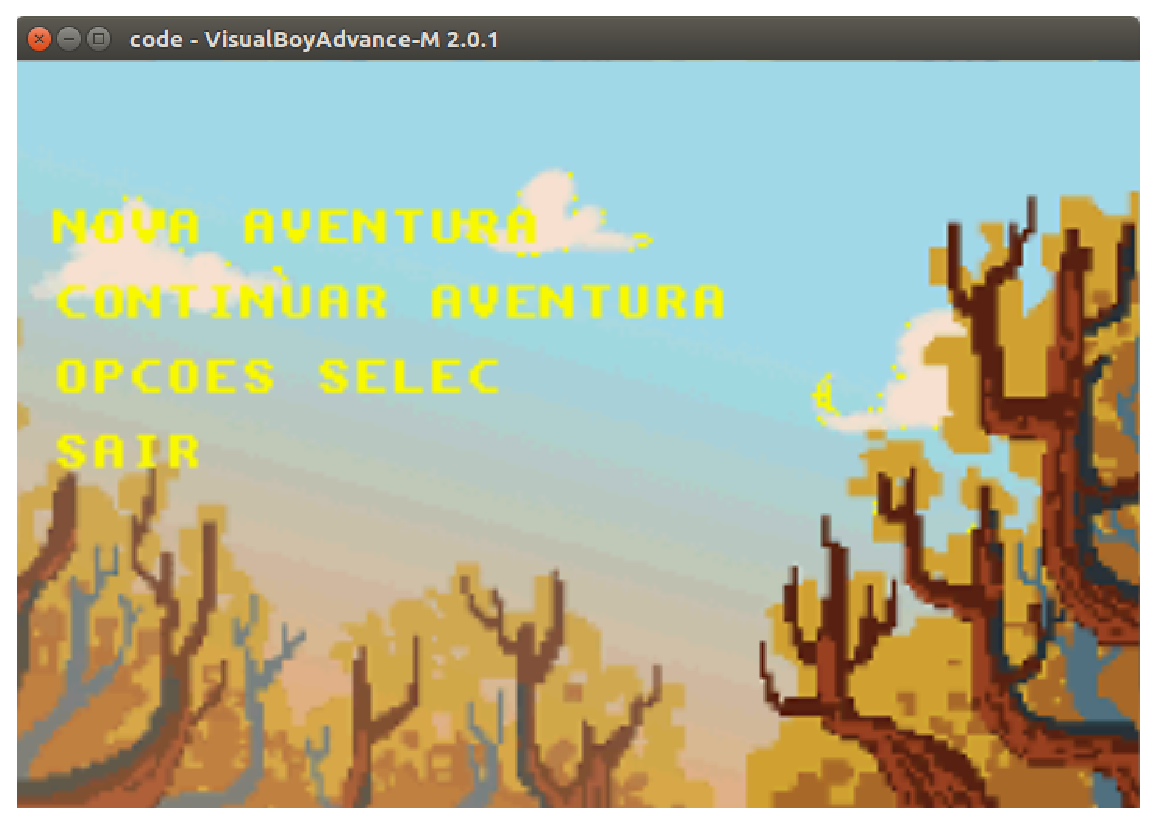
\includegraphics[width=16cm]{figuras/tw-gba-1.eps} }}%
    \caption{Comparação entre o jogo original e o protótipo no emulador.}%
    \label{fig:example}%
\end{figure}

Este protótipo inicial contém apenas a tela vista acima, com um \textit{background} desenhado ao fundo e quatro botões clicáveis, porém sem nenhuma ação após o clique. Para alterar o botão selecionado, basta

O protótipo desenvolvido está disponível no seguinte repositório: \url{https://github.com/traveling-will-gba/traveling-will-prototype}

\section{Desenvolvimento da \textit{engine}}

  Logo após a finalização do protótipo, foi iniciado o desenvolvimento da \textit{engine} responsável por substituir a \textit{libtonc} e gerenciar os recursos do jogo. Esta \textit{engine} contém os seguintes módulos: \textit{input}, vídeo, gerenciador de memória, áudio e física. Além disso, a \textit{engine} contém abstrações para os níveis (\textit{levels}) e objetos do jogo (\textit{game objects}) e um módulo utilitário para funções genéricas relacionadas ao \textit{hardware} do GBA.

  Os módulos de vídeo, \textit{input}, física e as abstrações para níveis e objetos do jogo foram desenvolvidos tendo como base a \textit{ijengine}\footnote{\textit{ijengine}, disponível em \url{https://github.com/fgagamedev/ijengine}}, \textit{engine} desenvolvida para a disciplina de Introdução aos Jogos Eletrônicos, que tem como foco a criação de jogos para PC utilizando \textit{C++}. Ela contém módulos de vídeo, áudio, manipulação de eventos, física, \textit{input}, dentre outros, e contém uma interface para a utilização de diferentes bibliotecas gráficas, como SDL\footnote{\textit{Simple DirectMedia Layer}, disponível em \url{https://www.libsdl.org}} e OpenGL\footnote{OpenGL, disponível em \url{https://www.opengl.org}}.

  \subsection{Módulo de \textit{input}}

Os estados dos botões do GBA ficam salvos em um registrador. Cada um desses estados é representado por um \textit{bit} do valor guardado por esse registrador. Sempre que um botão é pressionado, o GBA automaticamente troca o valor guardado nesse registrador de tal forma que o \textit{bit} que representa o botão em questão passe a possuir valor 0. De forma similar, quando o botão é solto, o valor contido no \textit{bit} em questão é modificado para 1, seu valor padrão. Sendo assim, a checagem dos estados pode ser realizada facilmente utilizando \textit{bitmasks}.

Por exemplo, caso se deseje checar um botão representado pelo \textit{bit} 2 (com a contagem começando em 0), basta pegar o resultado do \textit{AND} binário entre o valor guardado no registrador e a potência de 2 que possui como expoente o \textit{bit} em questão (4, nesse exemplo). No Código \ref{lst:input1} é possível visualizar a definição das constantes que representam os botões. A função utilizada para checar o estado de cada um deles pode ser vista no código \ref{lst:lalala}.

\begin{lstlisting}[caption={Cabeçalho do módulo de \textit{input}.},label={lst:input1}]
#ifndef INPUT_H
#define INPUT_H

#include <stdbool.h>
#include "base_types.h"

#define BUTTON_A 1
#define BUTTON_B 2
#define BUTTON_SELECT 4
#define BUTTON_START 8
#define BUTTON_RIGHT 16
#define BUTTON_LEFT 32
#define BUTTON_UP 64
#define BUTTON_DOWN 128
#define BUTTON_R 256
#define BUTTON_L 512
#define N_BUTTON 10

int pressed_state[N_BUTTON];

void check_buttons_states();
bool pressed(int button);

#endif
\end{lstlisting}

\begin{lstlisting}[caption={Código-fonte do módulo de \textit{input}.},label={lst:lalala}]
int pressed_state[N_BUTTON];
uint64_t key_update[N_BUTTON];
uint64_t update_counter;

void check_buttons_states() {
    update_counter++;

	for(int i = 0; i < N_BUTTON; i++) {
        int pressed = !((*buttons_mem) & (1 << i));

        if (pressed == pressed_state[i]) continue;

        pressed_state[i] = pressed;
        key_update[i] = update_counter;
	}
}

bool pressed(int button) {
	return pressed_state[32 - __builtin_clz(button) - 1] && key_update[32 - __builtin_clz(button) - 1] == update_counter;
}

bool pressing(int button) {
	return pressed_state[32 - __builtin_clz(button) - 1];
}
\end{lstlisting}

A Figura \ref{demo-input} apresenta o teste implementado para checar o pressionamento dos botões do GBA. Para cada botão pressionado um \textit{pixel} vermelho aparece na tela. Nesta figura, os botões B, R, \textit{LEFT}, \textit{DOWN} e \textit{START} estão sendo pressionados simultaneamente. O código \ref{lst:inputtest} apresenta este teste.

\begin{figure}[H]
 \centering 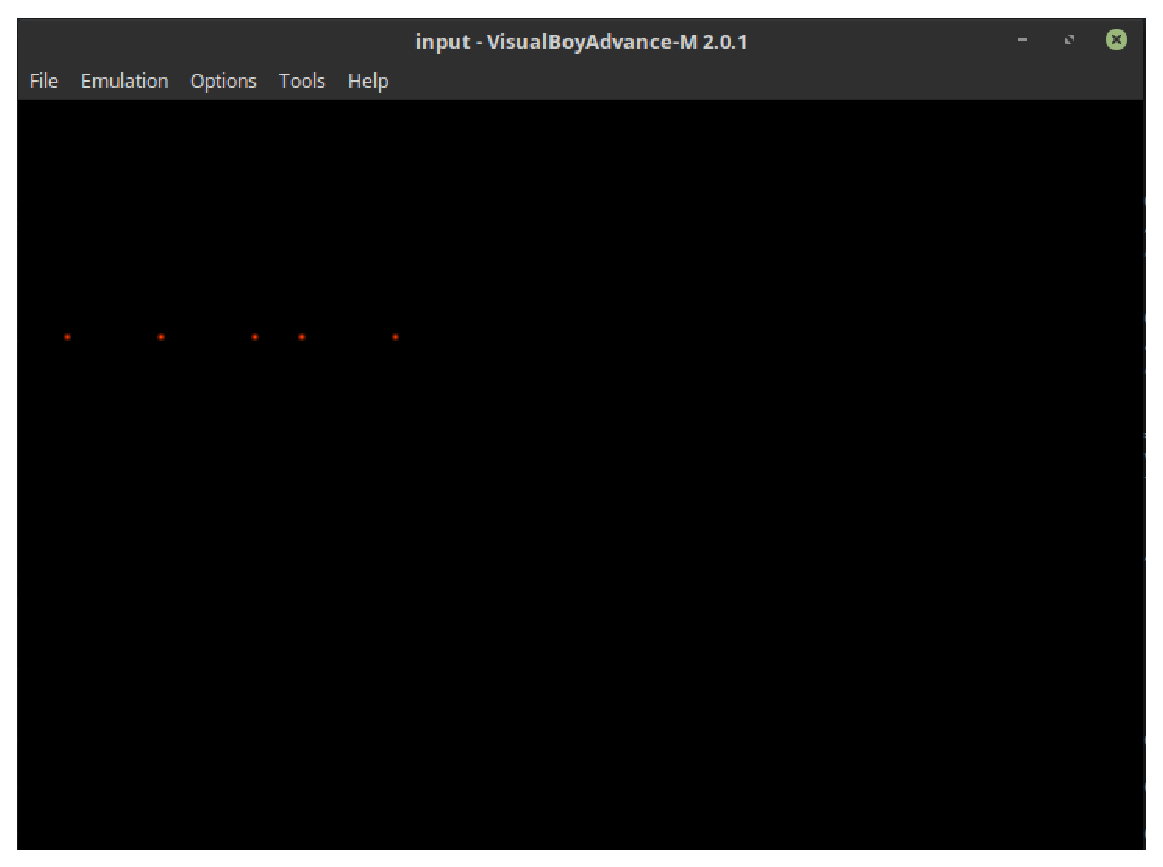
\includegraphics[keepaspectratio=true,scale=0.6]{figuras/demo-input.eps}
   \caption[Demonstração do pressionamento de botões no emulador]
    {Teste de pressionamento de botões no emulador.}
   \label{demo-input}
\end{figure}

\begin{lstlisting}[float,caption={Código de teste de \textit{input}.},label={lst:inputtest}]
#include "video.h"
#include "input.h"
#include "utils.h"

#define RED 0x0000FF

volatile unsigned short *vid_mem = (unsigned short *)0x6000000;

int main() {
	reset_dispcnt();
	set_video_mode(3);
	enable_background(2);

    while(1) {
        check_buttons_states();

        for(int i=0;i<=9;i++){
            int padding = i + 10;

            if (pressing(1 << i)) {
                for(int x=-2;x<=2;x++) {
                    for(int y=-2;y<=2;y++) {
                        vid_mem[(50 + x) * 240 + (20 + y + i * 10)] = RED;
                    }
                }
            }
            else {
                for(int x=-2;x<=2;x++) {
                    for(int y=-2;y<=2;y++) {
                        vid_mem[(50 + x) * 240 + (20 + y + i * 10)] = 0;
                    }
                }
            }
        }
    }

    return 0;
}
\end{lstlisting}

O código deste projeto se encontra no seguinte endereço: \url{https://bit.ly/2BQV6jf}.

  \subsection{Módulo de vídeo}

O módulo de vídeo é responsável pelo controle do modo de vídeo, dos \textit{backgrounds} e da renderização das \textit{sprites}.

Para gerenciar a renderização das \textit{sprites} foi desenvolvida uma classe chamada \textit{Texture}. Ela foi planejada de forma a não apenas copiar os dados da imagem para a região de memória apropriada, mas também permitir a animação das \textit{sprites} de uma textura e controlar os metadados das imagens renderizadas no jogo.

A seguir, será explicado, com o auxílo de trechos do código, o funcionamento dos principais elementos dessa classe.

Inicialmente, é necessário explicar os construtores dessa classe.

Logo abaixo, é possível visualizar o código do primeiro construtor. Ele recebe os ponteiros para a paleta de cores e para o vetor de \textit{tiles} utilizados pela imagem, os tamanhos das regiões de memória alocadas pra cada um desses ponteiros e a quantidade de \textit{bits} por \textit{pixel} que a imagem utiliza. Cada um desses atributos é guardado na própria classe, e, já nesse construtor, são chamados os métodos \textit{set\_sprite\_pal} e \textit{set\_sprite}, responsáveis por copiá-los para as regiões apropriadas. Por fim, ainda nesse construtor, são setados os índices do \textit{tile base} e da paleta de cores utilizada pela imagem. O cálculo desses índices será explicado logo adiante, nos tópicos dedicados aos métodos \textit{set\_sprite\_pal} e \textit{set\_sprite}.

\begin{lstlisting}[caption={Construtor da classe \textit{Texture}.}]
Texture::Texture(uint32_t num_sprites, const uint16_t *pallete, uint32_t pallete_len,
    const unsigned int *tiles, uint32_t tiles_len, enum bits_per_pixel bpp = _8BPP)
{
    this->pallete = pallete;
    this->pallete_len = pallete_len;
    this->pallete_id = 0;
    this->bpp = bpp;
    this->num_sprites = num_sprites;
    this->num_tiles = tiles_len / ((bpp == _4BPP) ? 32 : 64);
    this->tiles_per_sprite = num_tiles / num_sprites;
    this->tiles = tiles;
    this->tiles_len = tiles_len;

    memory_manager = MemoryManager::get_memory_manager();

    set_sprite_pal();
    set_sprite();
    oam_entry = memory_manager->alloc_oam_entry();

    metadata.tid = tile_base * ((bpp == _4BPP) ? 1 : 2);
    metadata.pb = pallete_id;
}
\end{lstlisting}
\vspace{\onelineskip}

O segundo construtor funciona de forma similar ao anterior, com a diferença de que em vez de receber todos os atributos da imagem, ele recebe apenas um ponteiro para outra textura. Esse construtor serve para quando se deseja renderizar réplicas de uma mesma textura. Utilizar ele permite que tais texturas compartilhem a paleta de cores e o vetor de \textit{tiles}, fazendo-se necessário alocar espaço apenas para os metadados, que são diferentes pra cada textura.

\begin{lstlisting}[caption={Construtor por cópia da classe \textit{Texture}.}]
Texture::Texture(const Texture *texture)
{
    this->num_sprites = texture->num_sprites;
    this->pallete = texture->pallete;
    this->pallete_len = texture->pallete_len;
    this->tiles = texture->tiles;
    this->tiles_len = texture->tiles_len;
    this->bpp = texture->bpp;
    this->pallete_id = texture->pallete_id;
    this->num_tiles = texture->num_tiles;
    this->tiles_per_sprite = texture->tiles_per_sprite;
    this->tile_base = texture->tile_base;

    memory_manager = MemoryManager::get_memory_manager();

    oam_entry = memory_manager->alloc_oam_entry();

    metadata.tid = tile_base * ((bpp == _4BPP) ? 1 : 2);
    metadata.pb = pallete_id;
}
\end{lstlisting}
\vspace{\onelineskip}

O método \textit{set\_sprite\_pal} é responsável por chamar o método \textit{alloc\_texture\_pal} da classe \textit{MemoryManager} passando como parâmetro o tamanho da paleta de cores a ser alocada. Como resultado, ele irá receber o endereço de memória aonde a paleta deverá ser guardada. Após fazer a cópia da paleta, é preciso calcular o índice da paleta escolhida na memória, já que esse é um dos metadados necessários para renderização da imagem a 4 \textit{bits} por \textit{pixel}. Como a região reservada para as paletas de cores no \textit{GBA} é divida em regiões de 32 \textit{bytes}, para realizar tal cálculo basta pegar a diferença entre o início da região escolhida para a cópia e o início da região reservada para as paletas e dividir por 32.
Como uma imagem renderizada a 8 \textit{bits} por \textit{pixel} ocupa toda a região reservada para as paletas, o cálculo do índice não é necessário para uma imagem que utilize 256 cores.

\begin{lstlisting}[caption={Função de alocação da paleta de cores de uma textura.}]
bool Texture::set_sprite_pal() {
    volatile uint8_t *teste = memory_manager->alloc_texture_palette(32);
    mem16cpy(teste, pallete, 32);

    this->pallete_id = (teste - (volatile uint8_t *)0x05000200) / 32;

    return true;
}
\end{lstlisting}
\vspace{\onelineskip}

O método \textit{set\_sprite} funciona de forma similar ao \textit{set\_sprite\_pal}, tendo como diferença relevante apenas o cálculo do índice do \textit{tile\_base} da imagem, que é feito subtraindo o início da região escolhida para a cópia e o início da região reservada para os \textit{tiles}. Essa diferença ocorre porque diferentemente da paleta de cores, cada unidade do vetor que representa a \textit{tile\_mem} no nosso código é, de fato, um \textit{tile}.

\begin{lstlisting}[caption={Função de alocação das \textit{sprites} de uma textura.}]
{c++}
bool Texture::set_sprite() {
    volatile struct tile *teste = memory_manager->alloc_texture(tiles_len);

    mem16cpy((volatile struct tile *)teste, tiles, tiles_len);
    tile_base = teste - memory_manager->base_texture_mem();

    return true;
}
\end{lstlisting}
\vspace{\onelineskip}

O método \textit{update\_metadata} apenas copia os metadados para a \textit{OAM} (\textit{Object Attributes Memory}).

\begin{lstlisting}[caption={Função de cópia dos metadados das texturas.}]
{c++}
void Texture::update_metadata() {
    mem16cpy(oam_entry, &metadata, sizeof(struct attr));
}
\end{lstlisting}
\vspace{\onelineskip}

Por fim, o método \textit{update} calcula qual a próxima sprite a ser renderizada e seta o primeiro \textit{tile} dela como \textit{tile\_id}. Esse processo é o que permite a animação das \textit{sprites} do jogo. O cálculo é feito somando o \textit{tile\_id} atual com a quantidade de \textit{tiles} por \textit{sprite} da textura que está sendo renderizada. Vale ressaltar que os índices dos \textit{tiles} são contabilizados sempre de 32 em 32 \textit{bytes}, mesmo que a imagem utilize 8 \textit{bits} por \textit{pixel} e por isso o número de \textit{tiles} por \textit{sprite} é multiplicado por 2 quando o número de \textit{bits} por \textit{pixel} da textura é 8.

Para a renderização dos \textit{backgrounds}, foi desenvolvida uma classe que recebe ponteiros para a paleta de cores,  para o vetor de \textit{tiles} e para o mapa de \textit{tiles} utilizados pelo \textit{background}, assim como os tamanhos das regiões alocadas pra cada um desses ponteiros. Assim que é instanciada, essa classe calcula qual o melhor \textit{charblock} e o melhor \textit{screenblock} para guardar os \textit{tiles} e o mapa de \textit{tiles}, respectivamente. Vale ressaltar que os \textit{charblocks} e \textit{screenblocks} compartilham a mesma região de memória e precisam de um espaço contíguo na memória do \textit{GBA} para que o \textit{background} seja renderizado corretamente. Por esse motivo não é recomendado apenas copiá-los para a memória do \textit{GBA} de forma sequencial, já que isso poderia causar um \textit{overlap} entre um \textit{charblock} e um \textit{screenblock}, e também poderia preencher a memória do \textit{GBA} de forma não-ótima, o que pode fazer com que não caibam todos os \textit{backgrounds} necessários para uma ou mais fases do jogo.

  \subsection{Módulo gerenciador de memória}

Para melhor utilização dos recursos providos pelo GBA foi desenvolvido um módulo que trata do gerenciamento de memória dos objetos do jogo. A principal responsabilidade deste módulo é garantir que a alocação e desalocação de recursos seja feita de forma eficiente e segura.

    \subsubsection{Funcionamento do gerenciador de memória}

    O modelo de gerenciamento escolhido para ser utilizado neste projeto foi o modelo de gerenciamento com partições variáveis \cite{tanenbaum}. Esse modelo se faz necessário pois os recursos a serem alocados durante a execução do jogo contém tamanhos distintos (uma sprite ocupa menos espaço que um \textit{background} que, por sua vez, ocupa menos espaço do que uma música). Além disso, é importante citar que este gerenciador aloca os recursos contiguamente na memória, isto é, ele sempre irá optar pelo primeiro espaço disponível a partir do começo da memória.

    Utilizando esse modelo como base, o gerenciador funciona da seguinte maneira:

    \begin{itemize}
        \item o construtor do gerenciador de memória é responsável por inicializar todos os ponteiros correspondentes aos endereços dos registradores de \textit{backgrounds}, texturas e atributos das texturas;
        \item quando ocorre uma chamada de alocação, o gerenciador procura pelo primeiro espaço disponível na memória correspondente para alocar tal recurso. Caso não ache nenhum espaço disponível, retorna um endereço nulo;
        \item após achar um endereço disponível, é verificado se há espaço suficiente para alocar o recurso. Caso não haja espaço suficiente, um endereço nulo é retornado;
        \item após garantir que há um espaço disponível e com espaço suficiente para alocação, a posição deste endereço no vetor auxiliar (responsável por indicar se determinado endereço está disponível ou não) é ligada (indicando que o espaço foi ocupado) e é retornado o endereço desta posição para o cliente (no caso, o jogo) realizar a cópia do recurso.
    \end{itemize}

    O código \ref{lst:alloc} apresenta a função responsável por realizar a alocação de paletas (tanto para \textit{backgrounds} quanto para texturas). Segundo \citeonline{gbatek}, as paletas possuem 256 entradas de 2 \textit{bytes}, totalizando 512 \textit{bytes}.

    \begin{lstlisting}[float,caption={Código de alocação de paletas para \textit{backgrounds} e texturas.},label={lst:alloc}]
    volatile uint8_t *MemoryManager::alloc_palette(bitset<512>& used,
        volatile uint8_t *palette, size_t size)
    {
        int used_size = used.size();

        for (size_t i = 0; i < used_size; i++) {
            // if this position is taken, skip it
            if (used[i] == true) {
                continue;
            }

            uint32_t available_pal_len = used_size - i;

            // if there is no space to allocate this pallete, skip it
            if (size > available_pal_len) {
                continue;
            }

            // mark positions from i to size as used
            for (size_t j = 0; j < size; j++) {
                used[i + j] = true;
            }

            memory_map[palette + i] = size;

            return palette + i;
        }

        return NULL;
    }
    \end{lstlisting}


    \subsubsection{Gerenciamento de memória}

    Para garantir que novos recursos sejam alocados e que nenhum objeto já carregado na memória seja sobrescrito ou corrompido, qualquer chamada que envolva a alocação de novos recursos passa por um processo onde é verificado se a memória que será populada contém espaço suficiente realizar tal alocação.

    Para realizar esta verificação, o gerenciador possui um mapa que associa um endereço na memória com o tamanho que o objeto alocado neste endereço ocupa. Deste modo, quando há uma chamada de alocação com tamanho \texttt{size} e uma posição \texttt{i} está disponível e o tamanho da partição em \textit{bytes} é dado por \texttt{t}, as posições de \texttt{i} até $ i + \frac{size}{t} - 1 $ são marcadas como utilizadas.

    As estratégias utilizadas para garantir um gerenciamento eficiente de memória envolvem a utilização de \textit{singleton} para a criação do objeto gerenciador de memória e utilização de estruturas de dados que permitam configurar o tamanho a ser utilizado.

    Para que haja um único objeto encarregado de gerenciar a alocação de recursos no jogo, a classe \texttt{MemoryManager} foi modelada utilizado o padrão de projeto \textit{Singleton}. Com este padrão de projeto, cada chamada de criação de uma nova instância do gerenciador de memória passa por uma verificação, que checa se já existe uma instância desta classe (por meio de uma variável dentro da própria classe que armazena uma instância de \texttt{MemoryManager} ou nulo). Caso haja, esta instância é retornada. Caso contrário, é criada uma nova instância. O código \ref{lst:manager} exemplifica o \textit{singleton} (trechos de código desta classe foram omitidos para melhor foco no padrão de projeto):

\begin{lstlisting}[caption={\textit{Singleton} do gerenciador de memória.},label={lst:manager}]
class MemoryManager {
    private:
        MemoryManager *instance;
    public:
        MemoryManager *get_memory_manager() {
            if (!instance) {
                instance = new MemoryManager();
            }
            return instance;
        }
};
\end{lstlisting}

A fim de não utilizar memória desnecessariamente, em alguns pontos do jogo foram utilizadas estruturas que permitem configurar a quantidade de \textit{bits} que podem ser utilizados por cada variável. O primeiro exemplo mostra uma \texttt{struct} que armazena os atributos das texturas, onde cada atributo só precisa de um pequeno número de \textit{bytes}. Já o segundo exemplo demonstra a utilização de \texttt{bitsets} (que mantém a disponibilidade de cada posição do endereço de memória) com tamanho fixo correspondente ao tamanho total da respectiva região de memória (neste exemplo, \texttt{Video RAM}).

\begin{lstlisting}[float,caption={\texttt{Struct} com \texttt{bitfields} para atributos das texturas.}]
struct attr {
    // attr0
    uint8_t y;
    uint8_t om : 2;
    uint8_t gm : 2;
    uint8_t mos : 1;
    uint8_t cm : 1;
    uint8_t sh : 2;
    // attr1
    uint16_t x : 9;
    uint8_t aid : 5;
    uint8_t sz : 2;
    // attr2
    uint16_t tid : 10;
    uint8_t pr : 2;
    uint8_t pb : 4;
    // attr3
    uint16_t filler;
};
\end{lstlisting}

\begin{lstlisting}[float,caption={\textit{Bitsets} para checagem de disponibilidade na memória.}]
// backgrounds and textures have 512 bytes each for palette memory
bitset<512> background_palette_used;
bitset<512> texture_palette_used;
// max number of charblocks that can be stored in VRAM
bitset<4> charblock_used;
// max number of screenblocks that can be stored in VRAM
bitset<32> screenblock_used;
\end{lstlisting}


  \subsection{Módulo de Física}

O módulo de física é responsável por checar continuamente se os objetos estão colidindo e caso estejam chamar as funções responsáveis por lidar com a colisão para cada objeto. Para realizar tal procedimento esse módulo guarda uma lista de objetos que devem ser considerados na checagem e um ponteiro para o objeto alvo. Dessa forma, sempre que algum objeto colide com o objeto alvo, o método \textit{on\_collision} do alvo e do objeto com o qual ele colidiu é chamado.


A \textit{engine} desenvolvida está disponível no seguinte repositório: \url{https://github.com/traveling-will-gba/gbengine}

  \subsection{Módulo Utilitário}

Este módulo contém funções utilitárias que estão relacionadas diretamente com \textit{hardware} do GBA.

A primeira delas é a função \texttt{print}. Esta função é necessária pois, diferentemente de um programa executado em um PC, a ROM não possui redirecionamento de \textit{output} para uma saída padrão. Após diversas buscas em fóruns de desenvolvimento para GBA, foi encontrada uma solução que permite realizar o redirecionamento do \textit{output buffer} para a saída padrão (\textit{stdin}). A solução consiste em um código \textit{Assembly} que contém uma chamada de sistema \texttt{vbaprint}. O código \ref{lst:vbaprint} apresenta a implementação \textit{Assembly} mencionada.

\begin{lstlisting}[label={lst:vbaprint}, caption={Código \textit{Assembly} para a função \texttt{vbaprint}}]
.arm
.global vbaprint
.type   vbaprint STT_FUNC
.text
vbaprint:
    swi 0xFF0000
        bx lr
\end{lstlisting}

Após isso é necessário declarar a função \texttt{vbaprint} em um cabeçalho em C. O código \ref{lst:vbaprintheader} apresenta este cabeçalho.

\begin{lstlisting}[label={lst:vbaprintheader}, caption={Cabeçalho da função \texttt{vbaprint}}]
#ifndef VBAPRINT_H
#define VBAPRINT_H

extern "C" void vbaprint(const char *message);

#endif
\end{lstlisting}

A implementação da função \texttt{print} utiliza o mesmo modelo de implementação da função \texttt{printf} da linguagem C. Ela recebe como parâmetros uma string e um \textit{wildcard} que indica que esta função recebe um número variável de parâmetros. Esse parâmetros variáveis são guardados em uma variável do tipo \texttt{va\_list}. Para realizar o \textit{parse} da \textit{string} recebida é utilizada a função \texttt{vsnprintf}, que recebe a lista de parâmetros e faz a resolução das variáveis na \textit{string} e retorna a string com as substituições feitas. Após isso, é chamada a função \texttt{vbaprint} que se encarrega de escrever o buffer recebido na saída padrão. O código \ref{lst:utilsprint} apresenta a implementação da função \texttt{print}.

\begin{lstlisting}[float,caption={Implementação da função \texttt{print}},label={lst:utilsprint}]
int print(const char *fmt, ...) {
    va_list args;
    va_start(args, fmt);

    char buffer[4096];

    int rc = vsnprintf(buffer, sizeof(buffer), fmt, args);

    vbaprint(buffer);
    va_end(args);

    return rc;
}
\end{lstlisting}

A próxima função utilitária é a \texttt{mem16cpy}. Esta função funciona de forma similar à função \texttt{memcpy} da linguagem C, porém, copia os dados de uma área de memória para outra 2 \textit{bytes} por vez. Isso se faz necessário pois

TODO

O código \ref{lst:mem16cpy} apresenta a implementação da função \texttt{mem16cpy}.

\begin{lstlisting}[caption={Implementação da função \texttt{mem16cpy}},label={lst:mem16cpy}]
void mem16cpy(volatile void *dest, const void *src, size_t n)
{
    if (n & 1) {
        print("Size must be even");
    }

    for (int i = 0; i < n / 2; i++) {
        *(((volatile uint16_t *)dest) + i) = *(((uint16_t *)src) + i);
    }
}
\end{lstlisting}

A última função deste módulo utilitário é a \texttt{vsync} (\textit{vertical synchronization}). Ela tem como responsabilidade servir como um mecanismo para garantir a atualização do jogo durante o período de VBlank (período onde há uma pausa na atualização vertical da tela do jogo). O código \ref{lst:vsync} apresenta a implementação do \texttt{vsync}.

\begin{lstlisting}[caption={Implementação da função \texttt{vsync}},label={lst:vsync}]
void vsync() {
    while(REG_VCOUNT >= 160);
    while(REG_VCOUNT < 160);
}
\end{lstlisting}

  \subsection{Abstrações de níveis e objetos do jogo}

Além de implementar módulos relacionados a entrada (\textit{input}) e saída (vídeo, áudio, entre outros), a \textit{engine} também implementa abstrações para os níveis e para os objetos do jogo.

Os \textit{game objects} são a base para qualquer elemento utilizado no jogo. Um \textit{game object} possui uma posição \texttt{(x, y)} no espaço do jogo, possui velocidade horizontal e vertical, possui \textit{game objects} filhos (que formam uma hierarquia de \textit{game objects}) e tem como responsabilidades atualizar seu próprio estado, se desenhar na tela e atualizar os seus filhos.

Pelo fato de o mecanismo de renderização ser, de certa forma, automático (basta carregar as imagens na memória e especificar os metadados que elas já são renderizadas na tela), a função de se desenhar na tela não é utilizada. Porém, a atualização e controle dos filhos é importante para o comportamento correto desses objetos. O código \ref{lst:gameobj} apresenta a classe \texttt{GameObject}.

\begin{lstlisting}[float,label={lst:gameobj},caption={Classe \texttt{GameObject}}]
#ifndef GAME_OBJECT_H
#define GAME_OBJECT_H

#include <vector>
#include <stdint.h>

using std::vector;

class GameObject {
    protected:
        GameObject *m_parent;
        int m_x, m_y;
        int m_speed_x, m_speed_y;
        vector <GameObject *> m_children;

        GameObject *parent() const { return m_parent; }

        virtual void update_self(uint64_t dt) = 0;
        virtual void draw_self() = 0;

    public:
        void update(uint64_t dt);
        void draw();

        void set_parent(GameObject *obj) { m_parent = obj; }
        void add_child(GameObject *);
        void remove_child(GameObject *);
};

#endif
\end{lstlisting}

Com a definição e implementação dos \textit{game objects}, a caracterização da abstração dos níveis do jogo se torna bem simples. De forma geral, um nível é um \textit{game object} que, além de possuir todas as propriedades já explicitadas acima, possui uma variável que indica se o nível foi finalizado e outra que guarda o próximo nível a ser renderizado. O código \ref{lst:level} apresenta a implementação da classe \texttt{Level}.

\begin{lstlisting}[label={lst:level},caption={Classe \texttt{Level}}]
#ifndef LEVEL_H
#define LEVEL_H

#include "game_object.h"

#include <stdio.h>

class Level : public GameObject {
    protected:
        int m_x, m_y;
        bool m_done;
        int m_next;
};

#endif
\end{lstlisting}

\section{Desenvolvimento do jogo}

  De acordo com o cronograma apresentado na versão anterior, as funcionalidades do jogo original que foram planejadas para a realização deste trabalho são:

  \begin{itemize}
    \item F1: implementação do menu principal do jogo
    \item F2: implementação da rolagem infinita dos \textit{backgrounds}
    \item F3: implementação do mecanismo de renderização das plataformas
    \item F4: implementação da movimentação do personagem principal
    \item F5: implementação do mecanismo de renderização dos itens coletáveis
    \item F6: implementação das telas de finalização dos níveis
    \item F7: carregamento dos níveis a partir do \textit{level design}
    \item F8: implementação do seletor de fases
    \item F9: implementação das opções do menu
    \item F10: implementação do tutorial
  \end{itemize}

  Da lista acima, as funcionalidades \texttt{F8}, \texttt{F9} e \texttt{F10} foram removidas da realização do projeto.

  O desenvolvimento do jogo foi marcado por quatro fases principais (que ocorreram simultaneamente): adaptação das imagens do jogo, construção dos níveis do jogo, transição entre os níveis do jogo e adaptação das músicas do jogo.

  \subsection{Adaptação das imagens do jogo}

Esta fase foi marcada principalmente pelo entendimento de como imagens são carregadas e interpretadas pelo GBA.

Primeiramente, era necessário conhecer a resolução das imagens no jogo original e no jogo a ser portado para que pudesse ser estabelecida uma proporção a ser utilizada na adaptação das imagens. Para isso, foram utilizadas as imagens de \textit{background}, pois elas ocupam todo o espaço da janela do jogo original. A altura dos \textit{backgrounds} no jogo original é \textit{480px} e, sabendo que a tela do GBA possui \textit{160px} o tamanho da tela do GBA é \textit{160px}, é possível estabelecer um fator de conversão bastante preciso, seguindo a fórmula

\begin{equation}
\label{Cálculo da proporção das imagens do jogo}
\frac{480_{px}}{160_{px}} = \frac{3}{1}
\end{equation}

Portanto, a proporção das imagens do jogo original para o jogo a ser portado é de \texttt{3:1}.

Após realizar o redimensionamento das imagens para o tamanho correto, foi necessário descobrir como utilizar essas imagens no GBA. Diferentemente de sistemas mais modernos, o GBA não carrega imagens de fato, e sim um código C que contém as informações da imagem, como paleta de cores, \textit{tiles} e o mapeamento desses \textit{tiles} na imagem. Para realizar a conversão da imagem para este código, foi utilizada a ferramenta GRIT (\textit{GBA Raster Image Transmogrifier}). Com essa ferramenta é possível converter a imagem utilizando uma série de parâmetros, como quantidade de bits por pixel da imagem, formato de redução de \textit{tiles}, formato de saída do arquivo gerado (C, \textit{Assembly}, entre outros), altura e largura, em \textit{tiles} (conjuntos de \textit{8px} x \textit{8px}), da imagem , dentre outras opções. Para a conversão das \textit{sprites} do jogo, o seguinte comando foi utilizado:

\begin{lstlisting}[language=bash,caption={Comando para conversão das imagens em código/}]
$ grit nome-da-imagem.png -gB4 -ftc -Mw2 -Mh4
\end{lstlisting}

Nesse commando, o código relativo à imagem é gerado a 4 \textit{bits} por \textit{pixel} (\textbf{-gb4}), exportando a imagem como código C (\textbf{-ftc}) e definindo a largura e a altura da imagem como sendo, respectivamente, \textit{16px} (\textbf{-Mw2}) e \textit{32px} (\textbf{-Mh4}). O resultado da execução dessa instrução é um \textit{header} e um código-fonte correspondentes à imagem, contendo uma paleta com as cores utilizadas e um vetor de tiles, assim como mostrado nos códigos \ref{lst:imageheader} e \ref{lst:imagecpp}.


\begin{lstlisting}[caption={\textit{Header} da parte superior da imagem da plataforma da primeira fase.},label={lst:imageheader}]
//{{BLOCK(level1_plat0)

//======================================================================
//
//  level1_plat0, 16x32@4,
//  Transparent palette entry: 17.
//  + palette 16 entries, not compressed
//  + 8 tiles Metatiled by 2x4 not compressed
//  Total size: 32 + 256 = 288
//
//  Time-stamp: 2018-11-28, 22:18:37
//  Exported by Cearn's GBA Image Transmogrifier, v0.8.15
//  ( http://www.coranac.com/projects/#grit )
//
//======================================================================

#ifndef GRIT_LEVEL1_PLAT0_H
#define GRIT_LEVEL1_PLAT0_H

#define level1_plat0TilesLen 256
extern const unsigned int level1_plat0Tiles[64];

#define level1_plat0PalLen 32
extern const unsigned short level1_plat0Pal[16];

#endif // GRIT_LEVEL1_PLAT0_H

//}}BLOCK(level1_plat0)
\end{lstlisting}

\begin{lstlisting}[caption={\textit{Código fonte} da parte superior da imagem da plataforma da primeira fase.},label={lst:imagecpp}]
//{{BLOCK(level1_plat0)

//======================================================================
//
//  level1_plat0, 16x32@4,
//  Transparent palette entry: 17.
//  + palette 16 entries, not compressed
//  + 8 tiles Metatiled by 2x4 not compressed
//  Total size: 32 + 256 = 288
//
//  Time-stamp: 2018-11-28, 22:18:37
//  Exported by Cearn's GBA Image Transmogrifier, v0.8.15
//  ( http://www.coranac.com/projects/#grit )
//
//======================================================================

const unsigned int level1_plat0Tiles[64] __attribute__((aligned(4))) __attribute__((visibility("hidden")))=
{
    0xCCCCCCCC,0xAAACCCCC,0x888AACCB,0x89988BBA,0x99889888,0x99898221,0x98822222,0x81122444,
    0xCCCCCCCC,0xCCCCCCBA,0xCCCCCA89,0xBB888989,0x78888988,0x25889988,0x44225889,0x22444168,
    0x22244223,0x44444444,0x44444444,0x44444444,0x44444444,0x44444444,0x44444444,0x44444444,
    0x44223432,0x44444244,0x44444444,0x44444444,0x44444444,0x44444444,0x44444444,0x44444444,
    0x44444444,0x44444444,0x44444444,0x43344334,0x24422222,0x42222222,0x22222222,0x22222222,
    0x44444444,0x44444444,0x44444444,0x33444344,0x44223432,0x22444244,0x22222222,0x11222222,
    0x22222222,0x21122222,0x11111111,0x11111111,0x11111111,0x11111111,0x11111111,0x11111111,
    0x11222222,0x11111122,0x11111111,0x11111111,0x11111111,0x11111111,0x11111111,0x11111111,
};

const unsigned short level1_plat0Pal[16] __attribute__((aligned(4))) __attribute__((visibility("hidden")))=
{
    0x0002,0x0889,0x088B,0x088D,0x10D0,0x092D,0x09AD,0x0A50,
    0x0A90,0x1290,0x0AD0,0x1332,0x1B74,0x0000,0x0000,0x0000,
};

//}}BLOCK(level1_plat0)
\end{lstlisting}

Já para a conversão dos \textit{backgrounds} foi utilizado o seguinte comando:

\begin{lstlisting}[language=bash,caption={Comando para conversão dos \textit{backgrounds} em código/}]
$ grit nome-da-imagem.png -gB4 -ftc -mRtf -mp0
\end{lstlisting}

Assim como na imagem anterior, ó código é gerado em C a 4 \textit{bits} por \textit{pixel}. Além disso, o código é gerado utilizando redução completa de \textit{tiles} (\textbf(-mRtf))  
Nesse commando, o código relativo à imagem é gerado a 4 \textit{bits} por \textit{pixel} (\textbf{-gb4}), exportando a imagem como código C (\textbf{-ftc}) e definindo a largura e a altura da imagem como sendo, respectivamente, \textit{16px} (\textbf{-Mw2}) e \textit{32px} (\textbf{-Mh4}). O resultado da execução dessa instrução é um \textit{header} e um código-fonte correspondentes à imagem, contendo uma paleta com as cores utilizadas e um vetor de tiles, assim como mostrado nos códigos \ref{lst:imageheader} e \ref{lst:imagecpp}.


\begin{lstlisting}[caption={\textit{Header} da parte superior da imagem da plataforma da primeira fase.},label={lst:imageheader}]
//{{BLOCK(level1_plat0)



  \subsection{Construção dos níveis do jogo}

  \subsection{Transição entre os níveis do jogo}

  \subsection{Adaptação das músicas do jogo}

Para que fosse possível carregar as músicas no GBA, foi necessário reduzir a frequência dos audios originais, técnica conhecida como \textit{downsampling}. No processo de redução, a qualidade dos sons diminui de forma considerável. Após gerar um novo arquivo \textit{.wav} com a frequência reduzida, o arquivo é convertido para o formato \textit{.mod}, para que este, por sua vez, possa ser interpretado pelo GBA.
 
O código \ref{lst:sound-class} mostra o construtor da classe \texttt{Sound}, responsável por inicializar a música e deixá-la pronta para ser tocada; o método \texttt{get\_sound}, que implementa o padrão \textit{singleton} e retorna a instância da classe; e o método \texttt{play}, responsável por tocar a música. Os métodos dessa classe apenas encapsulam funções já existentes na \textit{libgba}. 

\begin{lstlisting}[caption={Classe \texttt{Sound}},label={lst:sound-class}]
Sound* Sound::instance;

Sound::Sound() {
    irqInit();

    irqSet( IRQ_VBLANK, mmVBlank );
    irqEnable(IRQ_VBLANK);

    mmInitDefault( (mm_addr)soundbank_bin, 8); 
    mmStart( MOD_MUSIC43K, MM_PLAY_LOOP );
}

Sound *Sound::get_sound() {
    if (!instance) {
        instance = new Sound();
    }   

    return instance;
}

void Sound::play() {
    mmFrame();
}
\end{lstlisting}


  \subsection{Comparação entre o porte e o jogo original}

Esta Seção tem como objetivo comparar resultado final do porte do jogo com o jogo original. O jogo portado para GBA pode ser encontrado no seguinte endereço: \url{https://bit.ly/2RwXXDe}.

\clearpage

\begin{figure}%
    \centering
    \subfloat[Menu original.]{{\includegraphics[width=12cm]{figuras/comparacao/pc-menu.eps} }}%
    \qquad
    \subfloat[Menu portado.]{{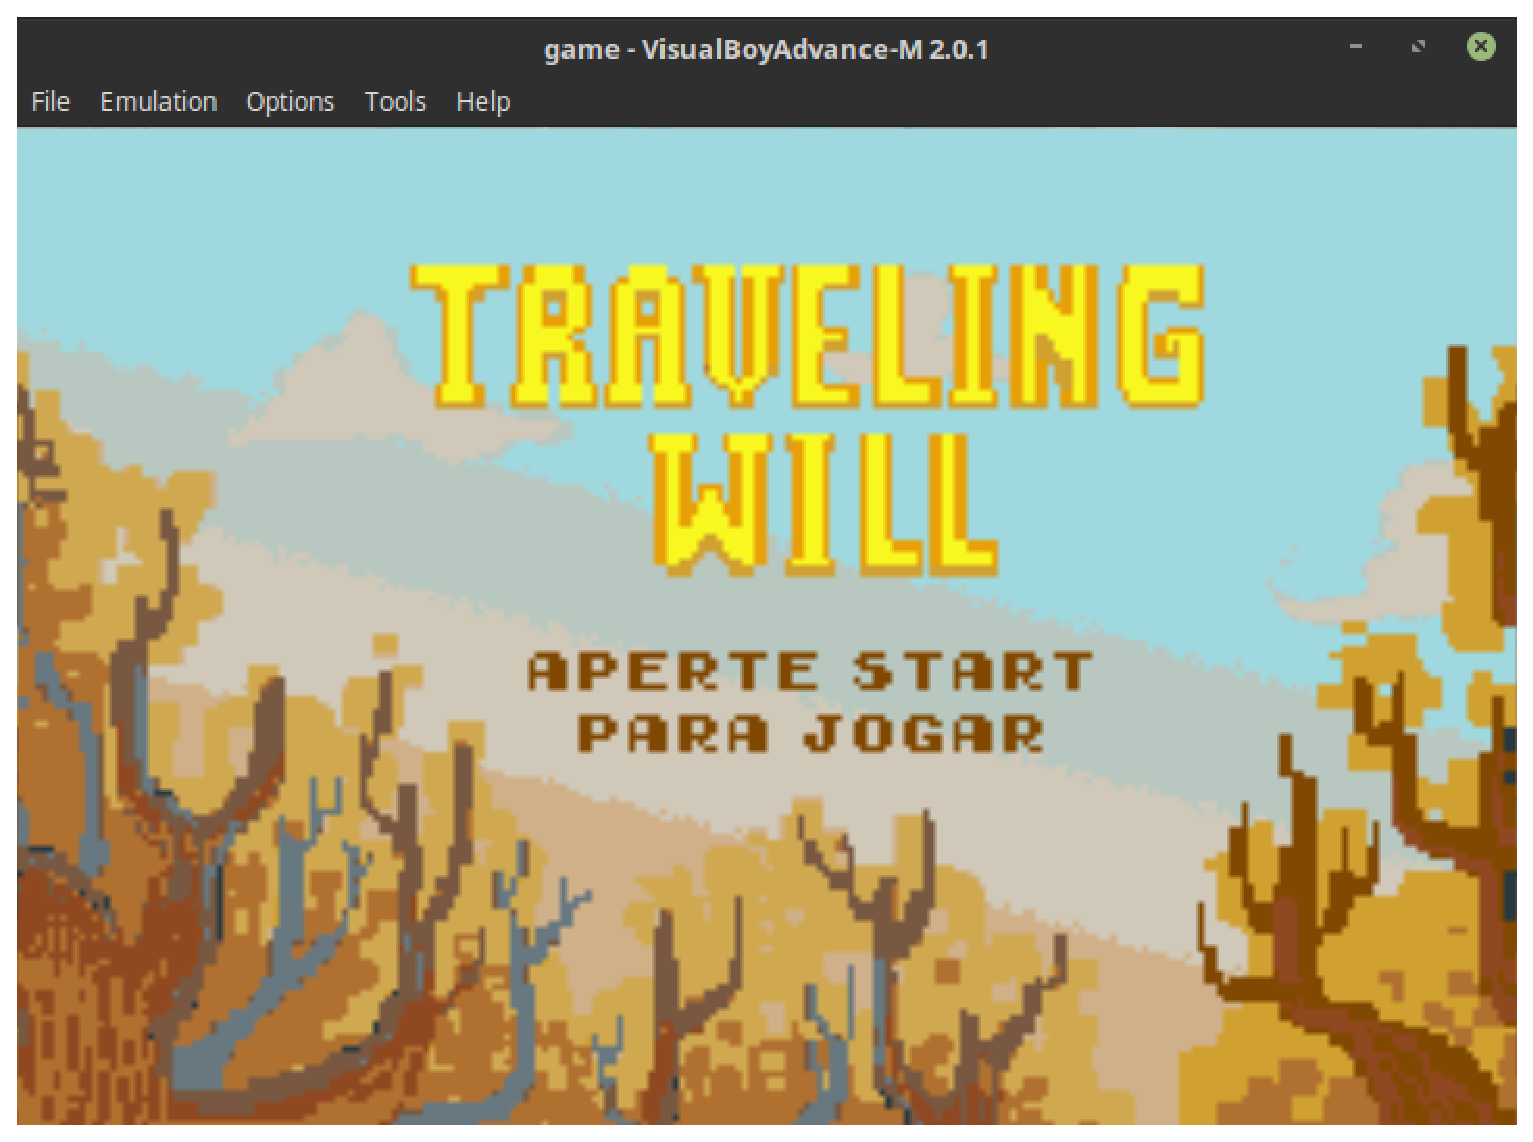
\includegraphics[width=12cm]{figuras/comparacao/gba-menu.eps} }}%
    \caption{Comparação do menu principal.}%
    \label{fig:example}%
\end{figure}

\begin{figure}%
    \centering
    \subfloat[Primeira fase original.]{{\includegraphics[width=12cm]{figuras/comparacao/pc-fase1.eps} }}%
    \qquad
    \subfloat[Primeira fase portada.]{{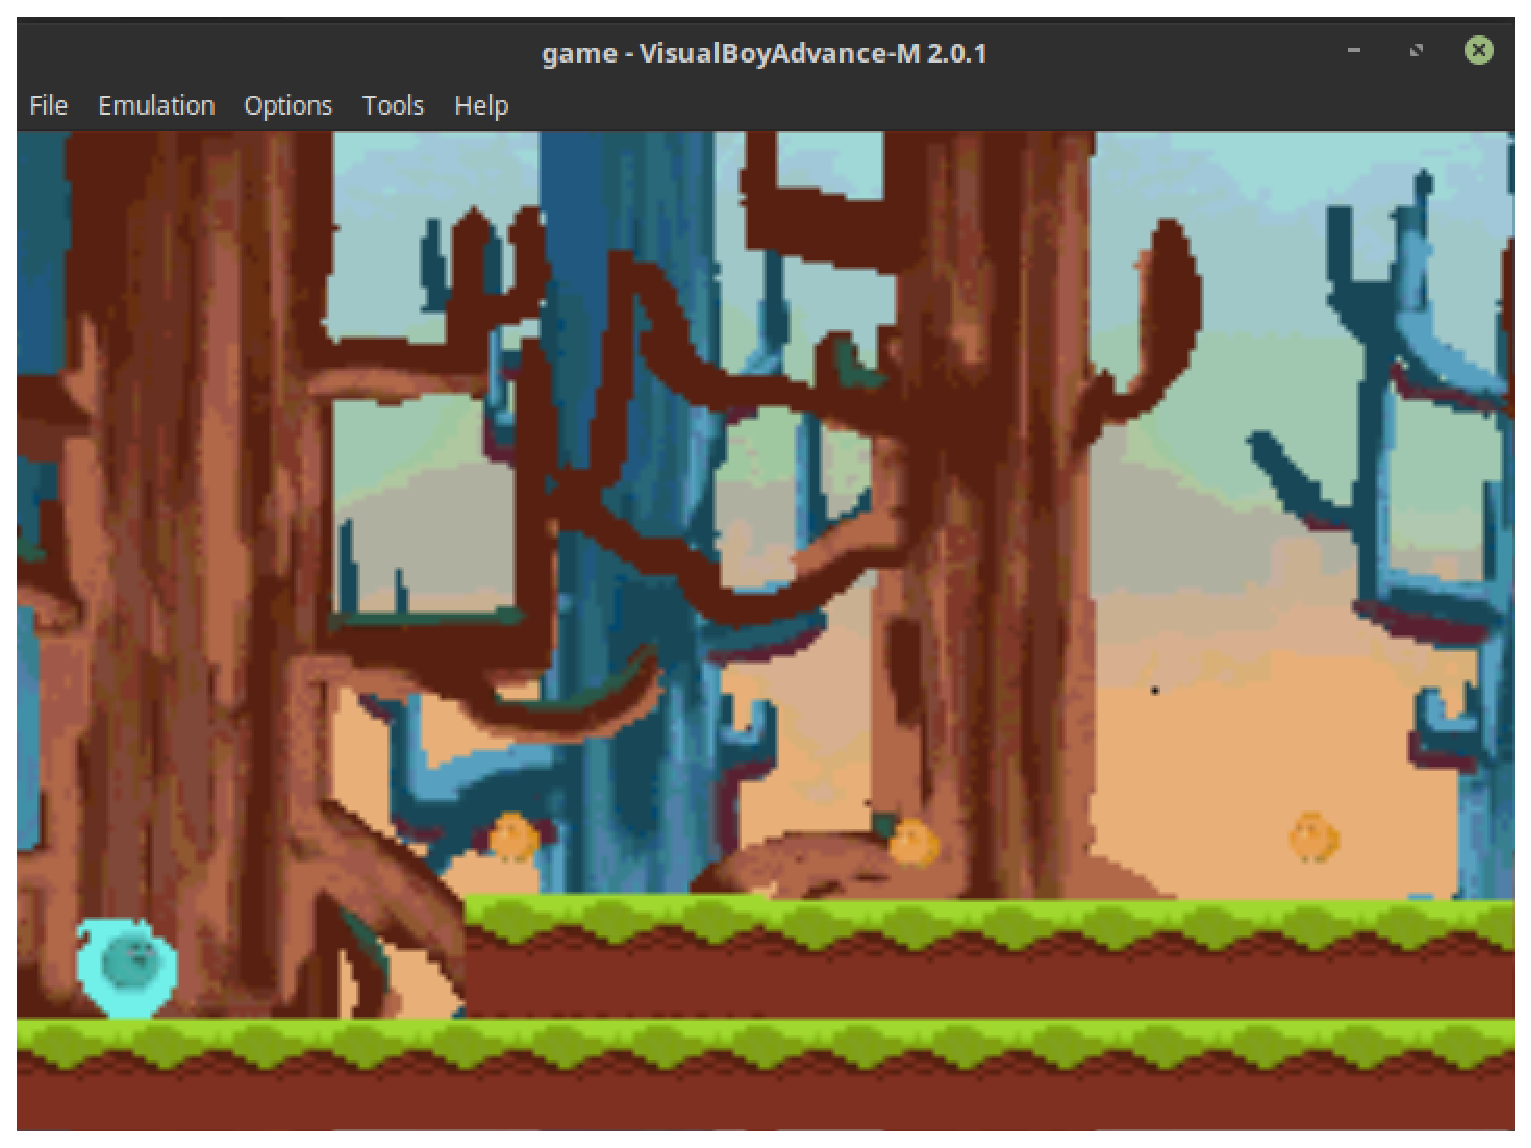
\includegraphics[width=12cm]{figuras/comparacao/gba-fase1.eps} }}%
    \caption{Comparação da primeira fase.}%
    \label{fig:example}%
\end{figure}

\begin{figure}%
    \centering
    \subfloat[Segunda fase original.]{{\includegraphics[width=12cm]{figuras/comparacao/pc-fase2.eps} }}%
    \qquad
    \subfloat[Segunda fase portada.]{{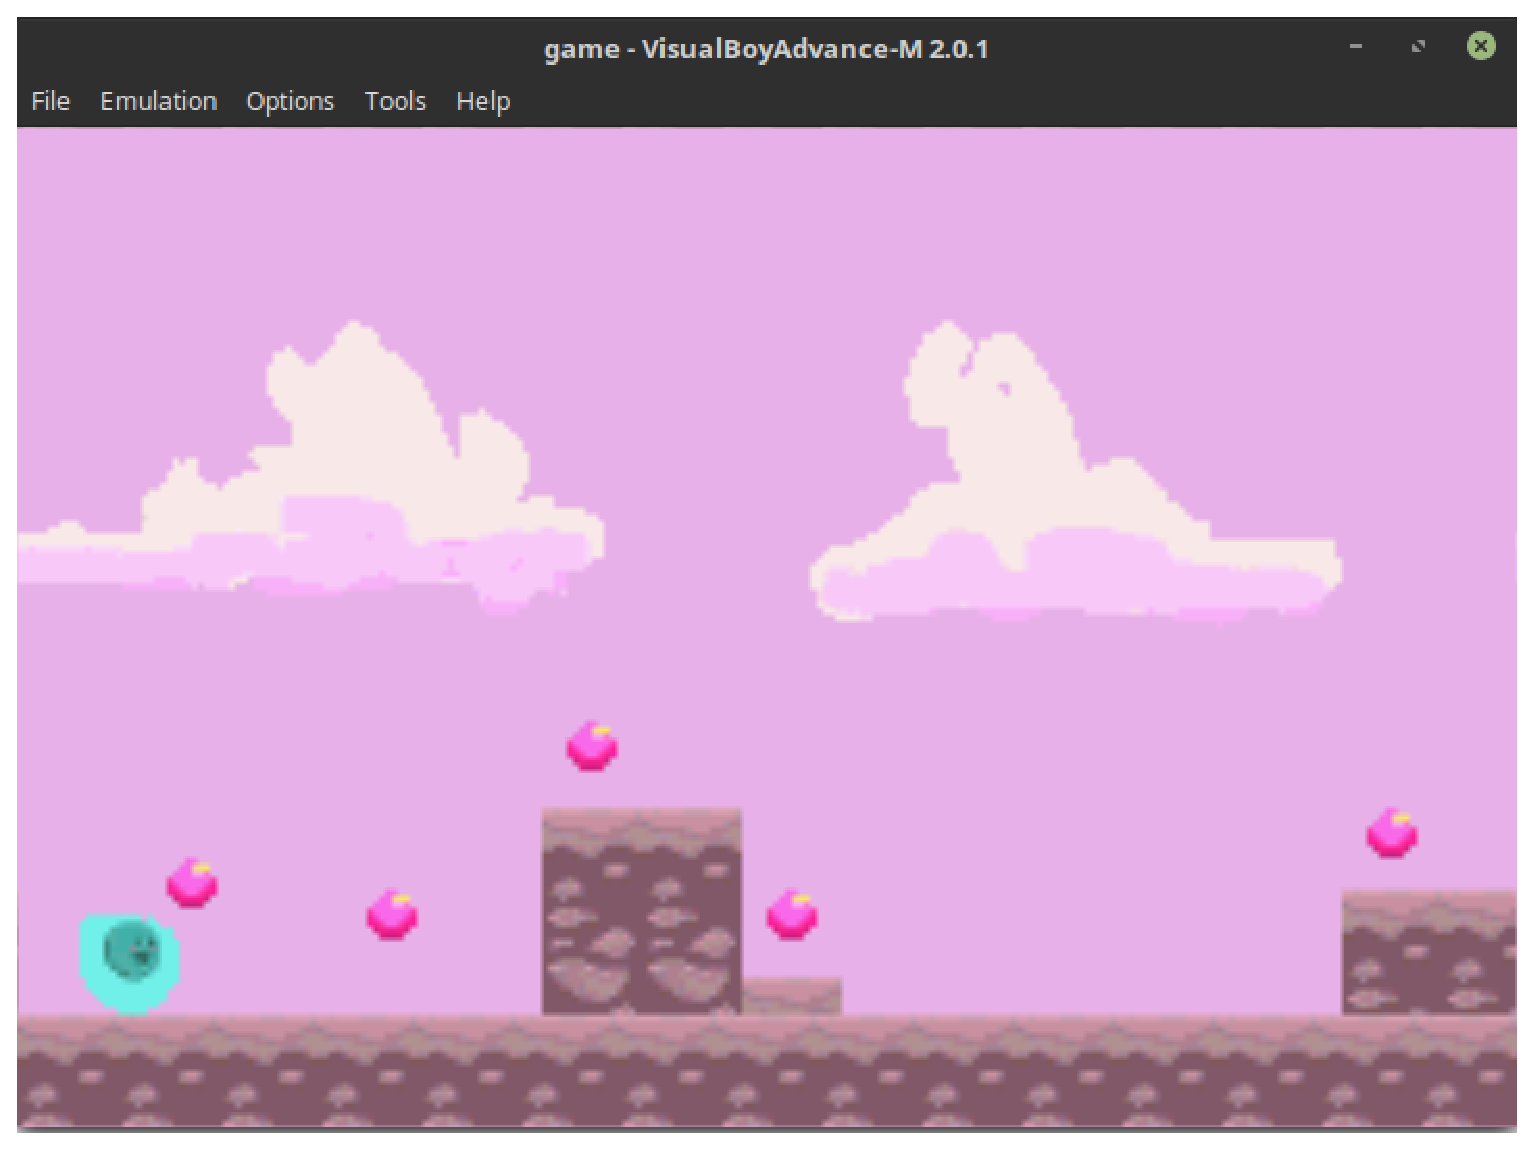
\includegraphics[width=12cm]{figuras/comparacao/gba-fase2.eps} }}%
    \caption{Comparação da segunda fase.}%
    \label{fig:example}%
\end{figure}

\begin{figure}%
    \centering
    \subfloat[Terceira fase original.]{{\includegraphics[width=12cm]{figuras/comparacao/pc-fase3.eps} }}%
    \qquad
    \subfloat[Terceira fase portada.]{{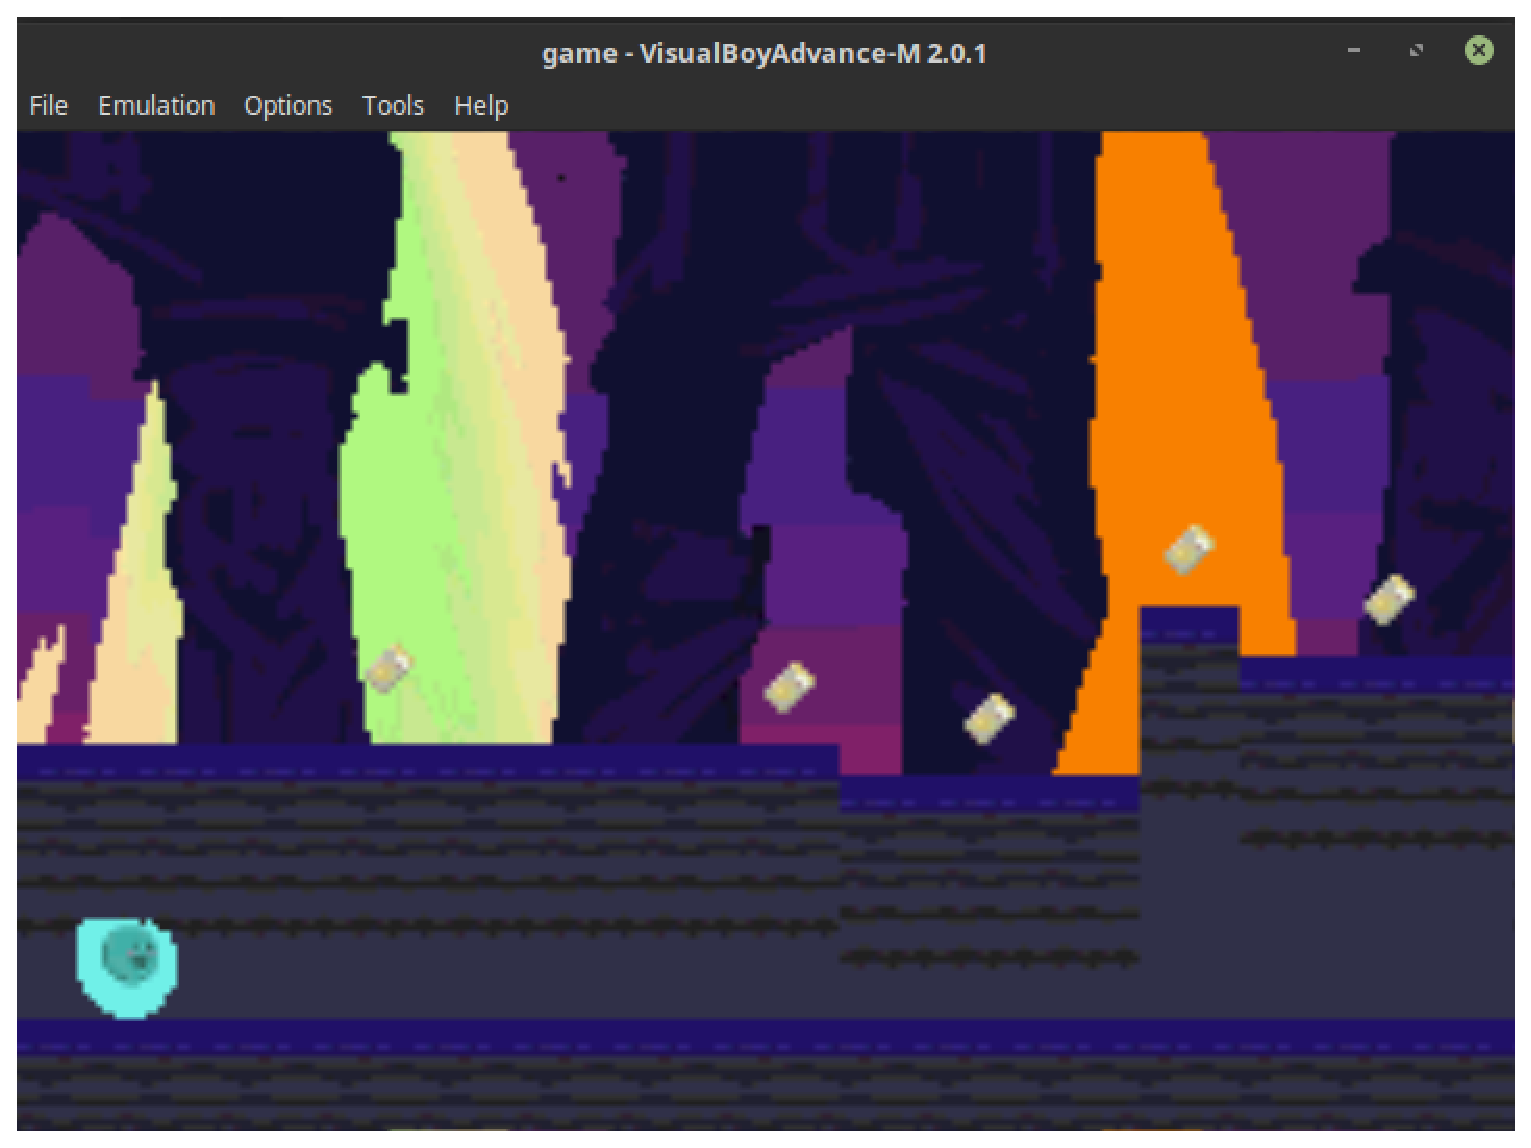
\includegraphics[width=12cm]{figuras/comparacao/gba-fase3.eps} }}%
    \caption{Comparação da terceira fase.}%
    \label{fig:example}%
\end{figure}

\begin{figure}%
    \centering
    \subfloat[Quarta fase original.]{{\includegraphics[width=12cm]{figuras/comparacao/pc-fase4.eps} }}%
    \qquad
    \subfloat[Quarta fase portada.]{{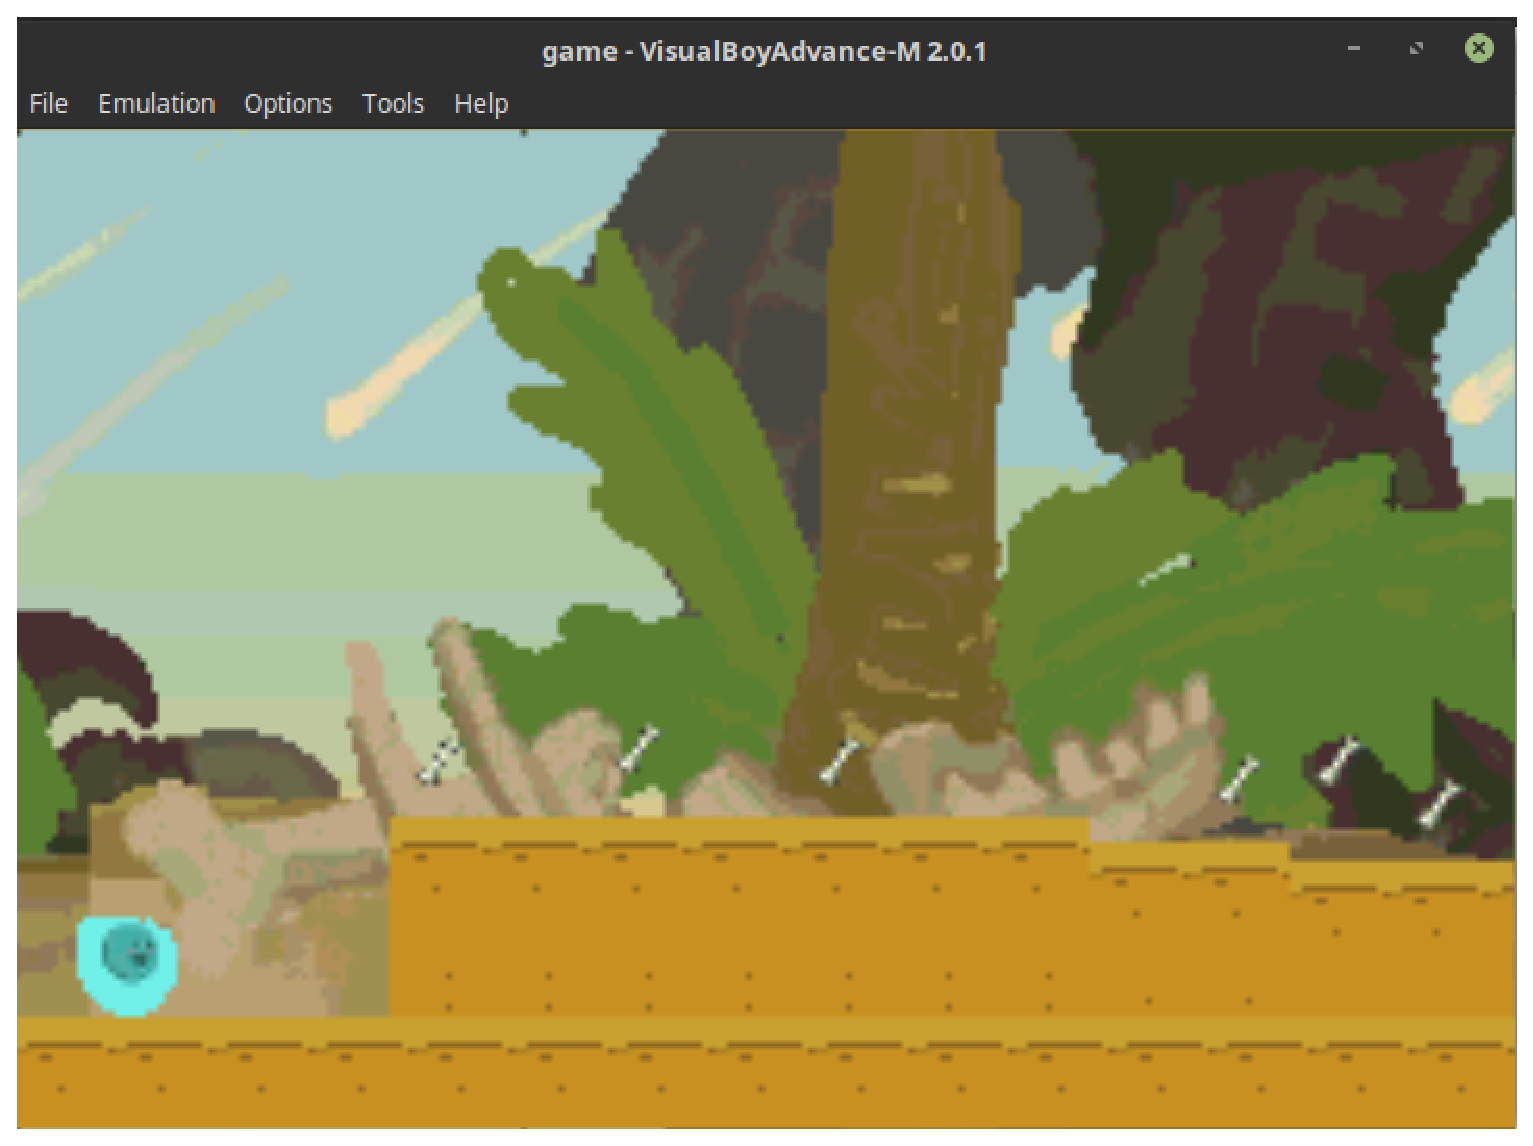
\includegraphics[width=12cm]{figuras/comparacao/gba-fase4.eps} }}%
    \caption{Comparação da quarta fase.}%
    \label{fig:example}%
\end{figure}

\begin{figure}%
    \centering
    \subfloat[Quinta fase original.]{{\includegraphics[width=12cm]{figuras/comparacao/pc-fase5.eps} }}%
    \qquad
    \subfloat[Quinta fase portada.]{{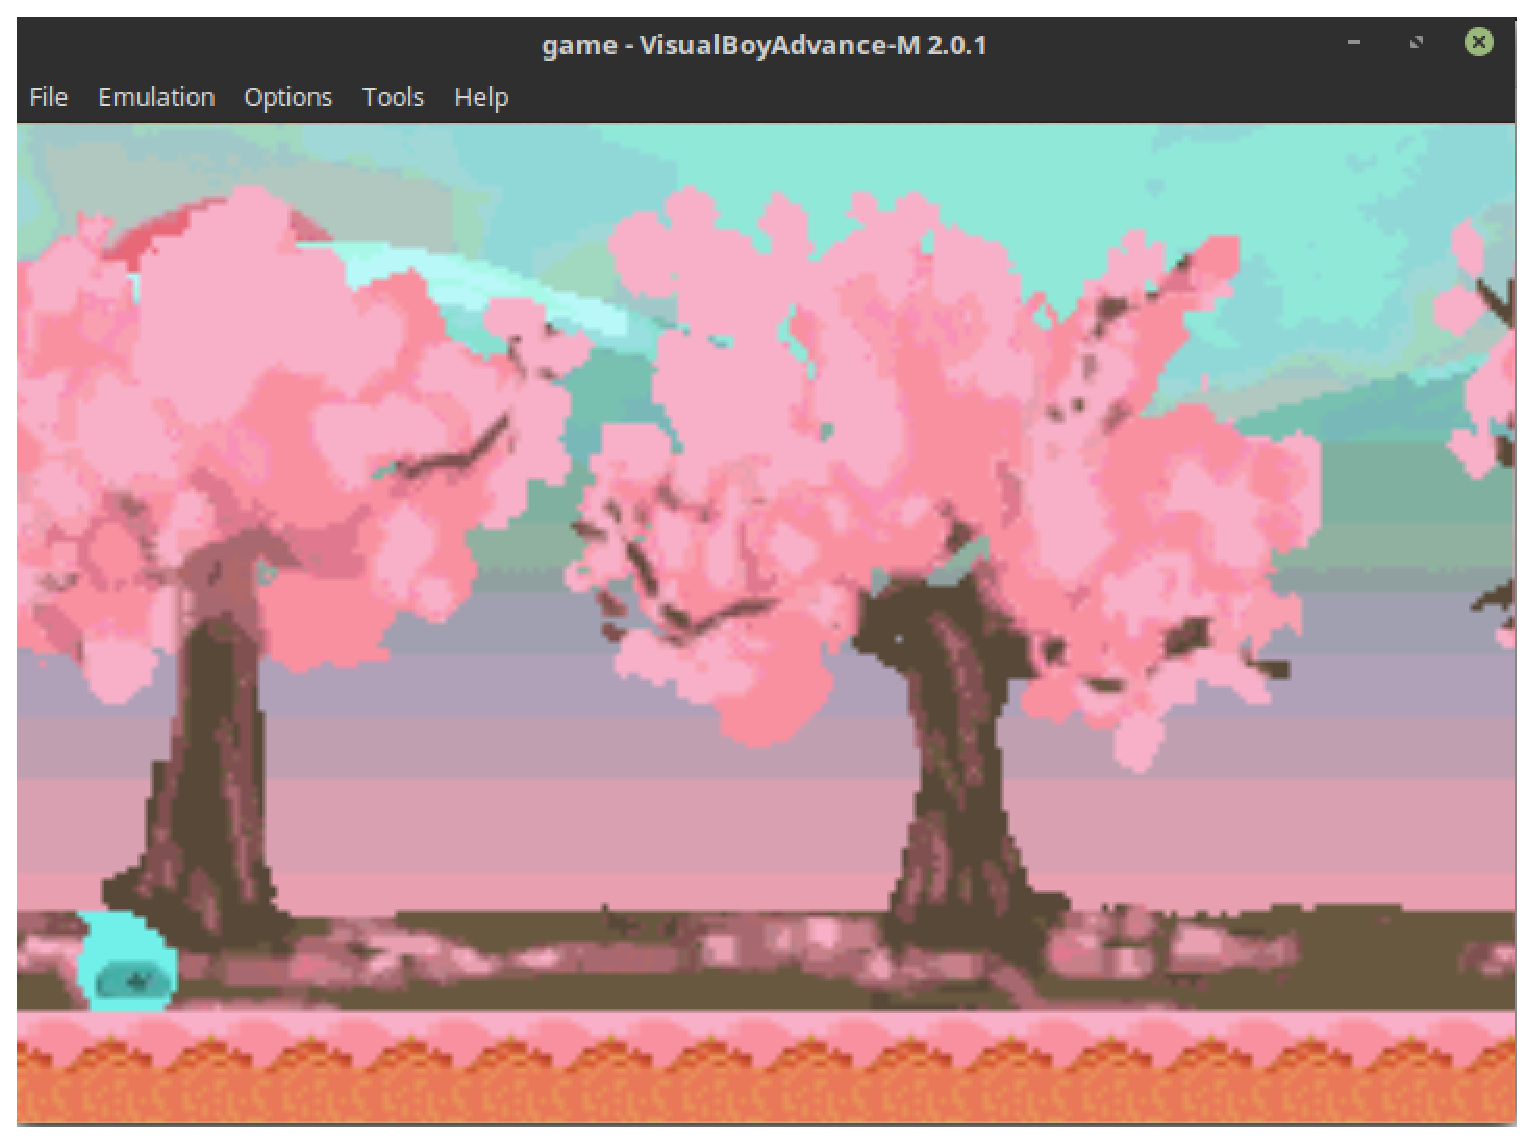
\includegraphics[width=12cm]{figuras/comparacao/gba-fase5.eps} }}%
    \caption{Comparação da quinta fase.}%
    \label{fig:example}%
\end{figure}

\begin{figure}%
    \centering
    \subfloat[Sexta fase original.]{{\includegraphics[width=12cm]{figuras/comparacao/pc-fase6.eps} }}%
    \qquad
    \subfloat[Sexta fase portada.]{{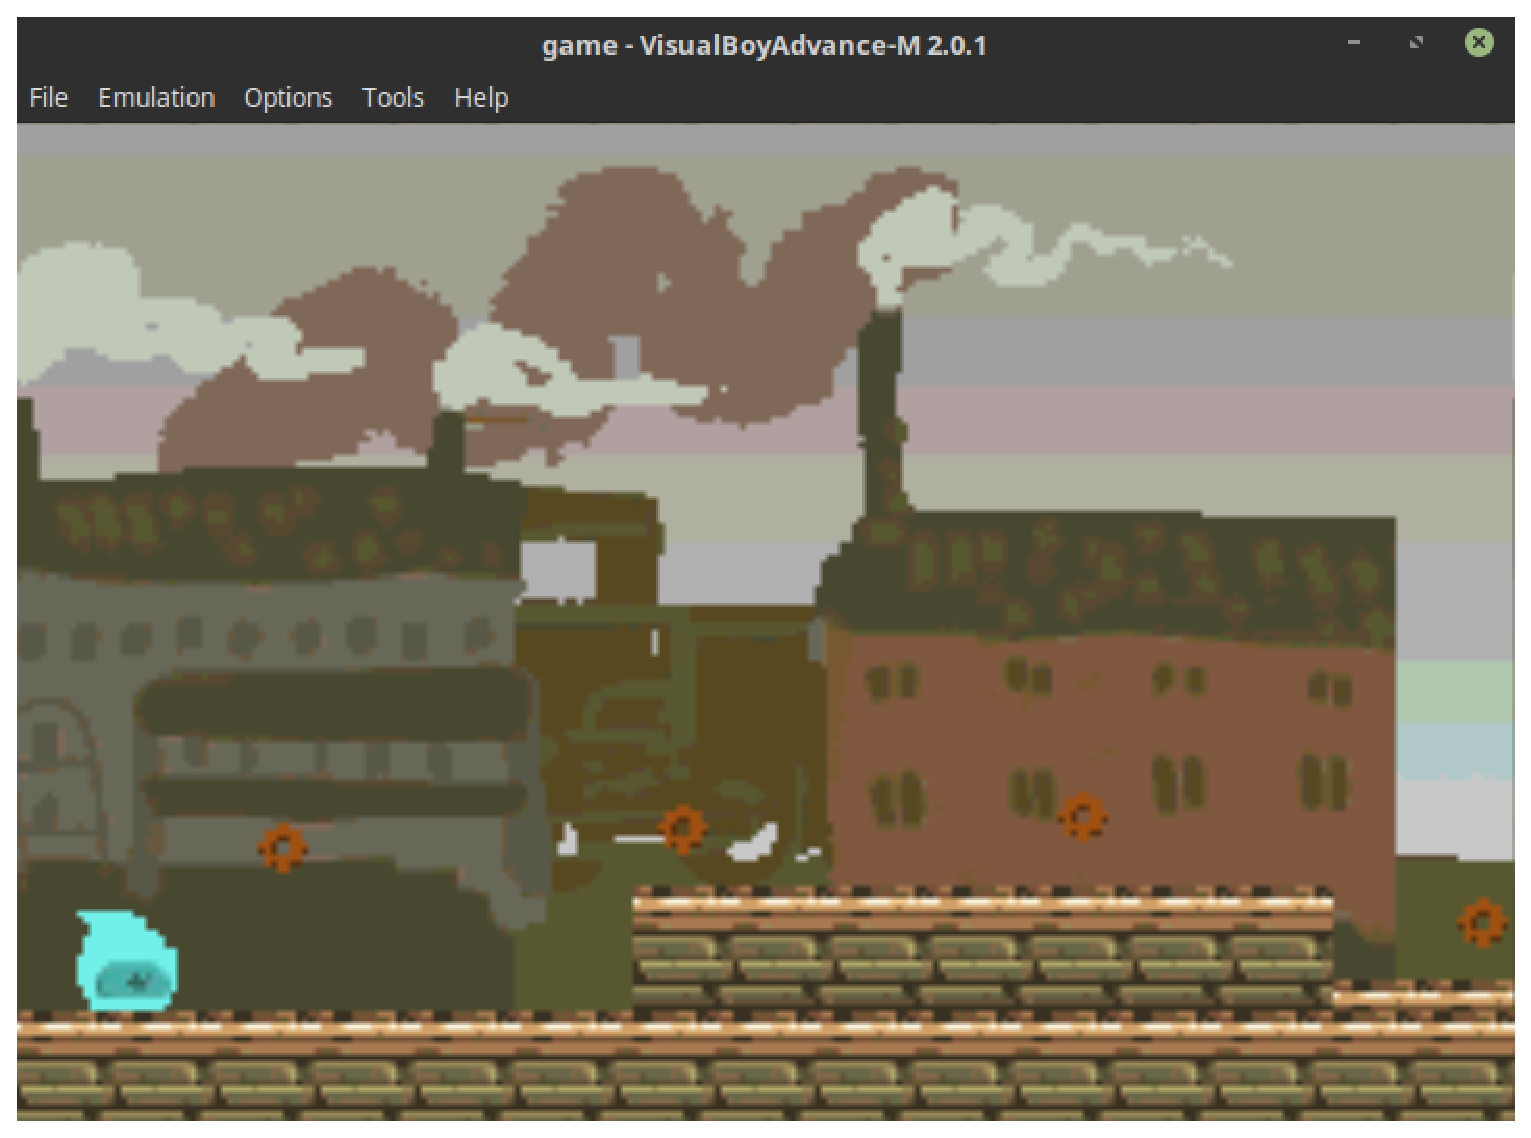
\includegraphics[width=12cm]{figuras/comparacao/gba-fase6.eps} }}%
    \caption{Comparação da sexta fase.}%
    \label{fig:example}%
\end{figure}

\begin{figure}%
    \centering
    \subfloat[Menu de vitória original.]{{\includegraphics[width=12cm]{figuras/comparacao/pc-vitoria.eps} }}%
    \qquad
    \subfloat[Menu de vitória portado.]{{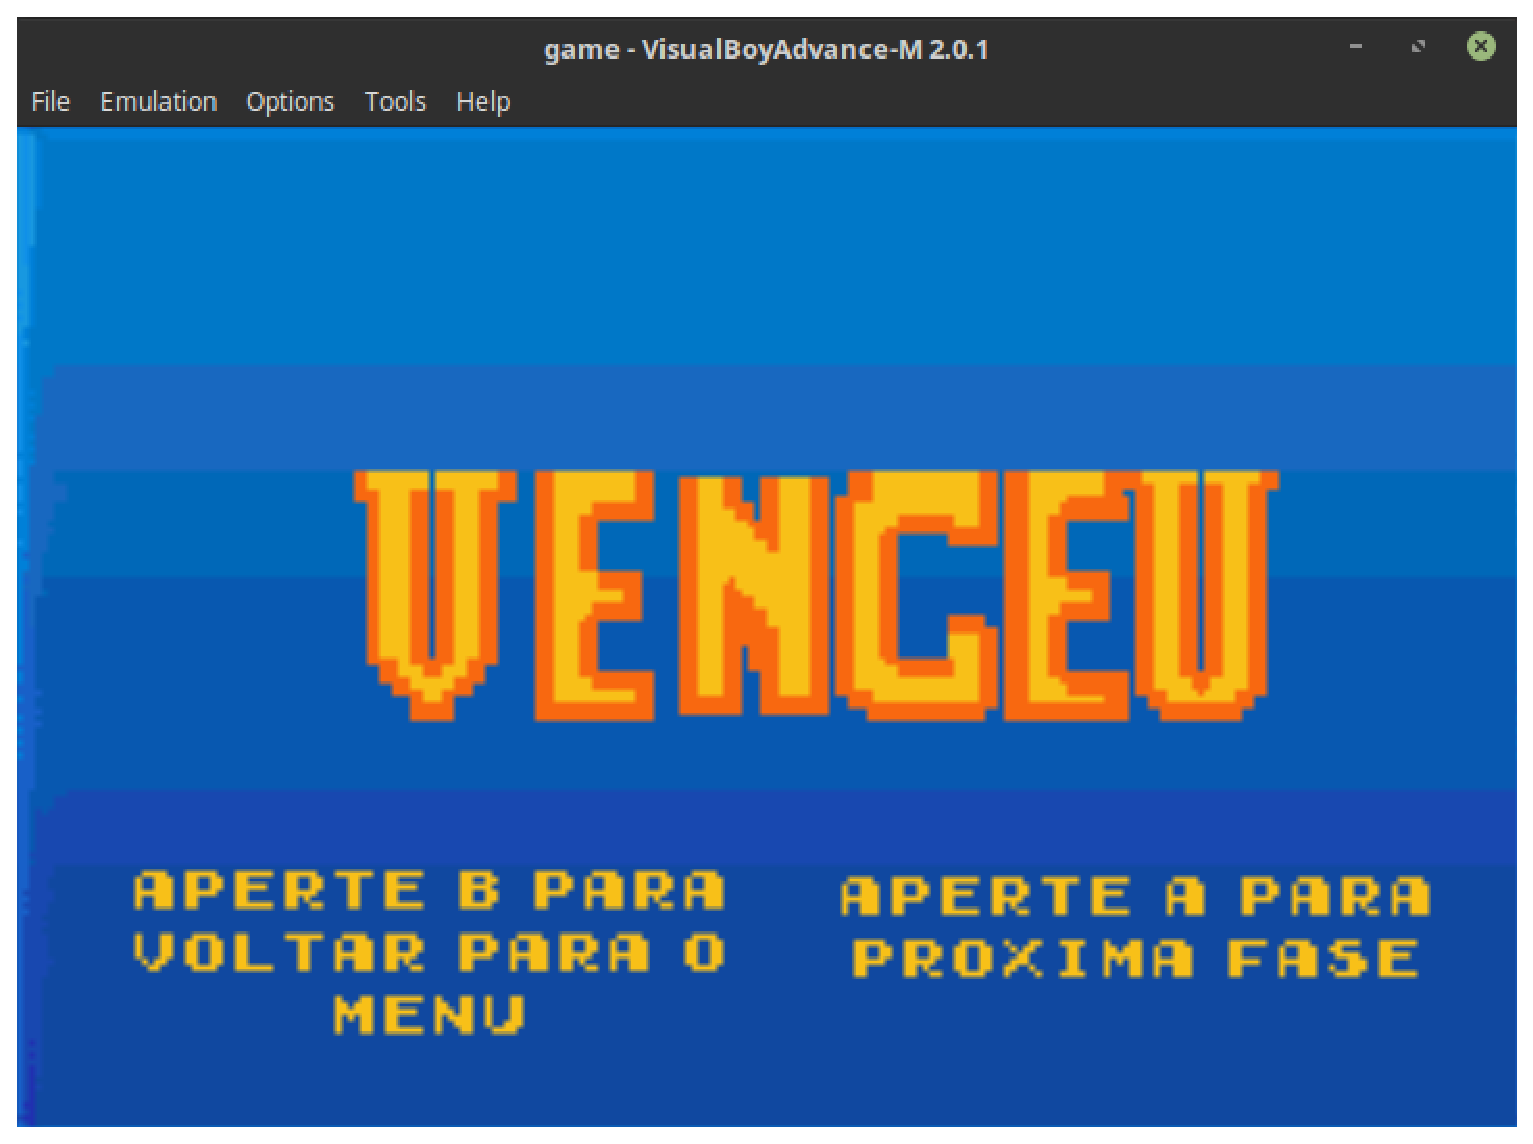
\includegraphics[width=12cm]{figuras/comparacao/gba-vitoria.eps} }}%
    \caption{Comparação do menu de vitória.}%
    \label{fig:example}%
\end{figure}

\begin{figure}%
    \centering
    \subfloat[Menu de derrota original.]{{\includegraphics[width=12cm]{figuras/comparacao/pc-defeat.eps} }}%
    \qquad
    \subfloat[Menu de derrota portado.]{{\includegraphics[width=12cm]{figuras/comparacao/gba-defeat.eps} }}%
    \caption{Comparação do menu de derrota.}%
    \label{fig:example}%
\end{figure}

% - adaptações em relação ao jogo original
%   - não possui opção para configurar o áudio durante o jogo
%   - não possui mecanismo de salvamento de dados do jogo
%   - não possui inimigos (ainda dá)
%   - não possui seletor de fase
%     - as fases são jogadas em ordem
%     - é possível pular de fase pressionando SELECT

% - transformar as imagens do jogo (Adaptação das imagens do jogo)
%   - proporção 3:1
%   - paleta de 15 cores
%     - bit 0 transparente, mas o grit não faz isso certo
%     - especificar comandos do grit gerados para backgrounds e paletas
%   - backgrounds
%     - especificar paleta de cores na hora de gerar o grit
%     - como foi feito o scroll infinito dos backgrounds
%       - falar sobre os registradores
%   - texturas
%     - animação -> como foi feita
%     - plataformas -> uma plataforma contém várias sprites
%       - metadata.om = 2 para esconder as plataformas da tela (senão portal)
%         - colocar imagem do portal
%     - problemas com lixo na OAM, sprites espelhando

% - parse do level design (Construção de um nível do jogo)
%   - explicar como é o level design do traveling will
%   - explicar o que o parser gera e como ele é usado no jogo
%   - colocar código do parser python
%   - explicar o uso de fila para as plataformas (pouca memória)
%     - construtor por cópia
%   - velocidade das plataformas é dada pela velocidade do background mais a frente
%   - fim do level tudo para
%     - will se mexe

% - Transição entre níveis do jogo
%   - dois tipos de níveis (jogáveis e não-jogáveis)
%   - escolha do nível a ser construído
%     - switch case
%       - não era possível modularizar por causa das variáveis (inferência de nome)

% - Adaptação das músicas do jogo
%   - falar brevemente sobre os canais de áudio do gba e colocar referência
%   - falar que o módulo de áudio atual permite reproduzir notas únicas (ondas quadradas?)
%   - colocar código da reprodução da notas
%   - falar do parser do level design para extrair a música do level
%     - explicar o que ele gera
%   - colocar código do parser
%   - explicar que esse modelo não foi utilizado por era muito simples
%   - falar que o GBA consegue reproduzir apenas sons .mode
%   - falar sobre conversão de wav pra mod
%     - falar sobre a quantidade de bits do wav (colocar referência)
%     - conversão da quantidade de bits do wav
%     - conversão do wav pra mod (usando a ferramenta X)
%       - qualidade do som diminui bastante
%   - problemas em executar o nível e o áudio ao mesmo tempo
%     - sincronização da música com o level e velocidade do jogo

% - problemas gerais
%   - depuração de código
%     - rodar debuggers (gdb, etc)
%     - somente a base de print

% - o que não foi feito
%   - mixer sofisticado
%   - módulo de texto
%     - fontes bitmap mode + outras prioridades
%   - inimigos (ainda dá)
\chapter[Considerações finais]{Considerações finais}

Durante o desenvolvimento da \textit{engine} e do jogo, em diversos momentos bastante tempo foi empregado tentando entender detalhes da especificação do \textit{hardware} do GBA, como a definição da paleta de cores dos \textit{backgrounds} e \textit{sprites} serem bastante diferentes, o \textit{overlap} entre \textit{charblocks} e \textit{screenblocks} na região de memória VRAM, os diferentes canais de áudio que serviam para propósitos bem diferentes, a impossibilidade de se utilizar uma ferramenta de depuração de código, como \texttt{gdb}\footnote{\textit{GNU Debugger}, disponível em \url{https://bit.ly/2r2Wzza}}, entre outros.

Um dos maiores impedimentos desse trabalho foi a dificuldade em conseguir testar os jogos no \textit{console}. Essa dificuldade se deu principalmente pelo fato do cliente utilizado para realizar a transferência das ROM's possuir versão apenas para \textit{Windows XP}, sendo necessário utilizar uma máquina virtual apenas para esse processo, e pela sincronização entre o cliente e o dispositivo físico não ser constante, deixando de funcionar diversas vezes sem motivo aparente. Outro grande impedimento foi a conversão dos áudios para um formato adequado para o GBA. Após muita pesquisa, foram encontradas ferramentas que permitiam realizar tal conversão, mas que necessitavam que o \textit{sample rate} dos áudios fosse reduzido, ocasionando uma perda notável na qualidade final das músicas. 

Além dos problemas relacionados ao \textit{hardware} do GBA, adaptar os recursos do jogo original de forma que pudessem ser carregados no GBA e testar o jogo no \textit{console} foram outras situações que demandaram boa parte do tempo do desenvolvimento do jogo. A dificuldade em testar o jogo no \textit{console} se deu principalmente pelo fato do cliente utilizado para realizar a transferência das ROM's possuir versão apenas para \textit{Windows XP}, sendo necessário utilizar uma máquina virtual apenas para esse processo, e pela sincronização entre o cliente e o dispositivo físico não ser constante, deixando de funcionar diversas vezes sem motivo aparente. Outro grande impedimento foi a conversão dos áudios para um formato adequado para o GBA. Após muita pesquisa, foram encontradas ferramentas que permitiam realizar tal conversão, mas que necessitavam que o \textit{sample rate} dos áudios fosse reduzido, ocasionando uma perda notável na qualidade final das músicas. 

Durante o processo de desenvolvimento do jogo, foram encontrados pontos de melhoria em certas tarefas/ações. Um dos pontos seria realizar uma melhor priorização das tarefas a serem executadas (por exemplo, o módulo de áudio foi o último a ser implementado). Outro ponto seria aumentar a frequência de realização de testes do jogo no \textit{console}. Isso ajudaria a validar o impacto das melhorias no \textit{hardware} real, já que o emulador não necessariamente reproduz à risca o comportamento do GBA.

Como resultado do trabalho, não foi possível executar o jogo final no \textit{console}, devido às divergências entre o emulador e o GBA e ao fato de não termos realizado os testes com a frequência necessária, sem saber, portanto, o ponto aonde o jogo deixou de funcionar no \textit{console}, porém foi possível executar em emuladores para computador e até mesmo para celulares.

\section{Trabalhos futuros}

Como sugestões de trabalhos futuros, têm-se: Corrigir funcionamento do jogo no GBA, investigar impactos do uso da linguagem C++, melhorar módulo de áudio para permitir carregar efeitos sonoros e pausar músicas durante a execução do jogo, implementar carregamento e utilização de fontes no jogo, adicionar elementos de HUD e seleção de fases, salvar o estado do jogo em memória e implementar um desfragmentador de memória na classe \texttt{MemoryManager}.


\bookmarksetup{startatroot}

\postextual

\bibliography{bibliografia}
% \input{editaveis/apendices}
% \input{editaveis/anexos}
\printindex

\end{document}

